
\newcommand{\ourname}{BOLT}

\section{Abstract}
In this paper we introduce \ourname, a novel approach for the problem of energy disaggregation that performs online binary matrix factorization on a sequence of high frequency current cycles collected in a building to infer additive subcomponents of the current signal. The system learns these constituent current waveforms in an unsupervised fashion and, in a subsequent step, seeks to find combinations of these subcomponents that constitute appliances. By doing so, points in time when appliances are active and, to some degree, their power consumption can be estimated by \ourname. Our system treats energy disaggregation as a binary matrix factorization problem and uses a neural network, with binary activations in the one but last layer and a linear output layer, to solve it. The algorithmic performance of the proposed method is evaluated on a publicly available dataset. Furthermore, we show that, once the model is trained, the algorithm can perform inference in real-time on inexpensive off-the-shelf and general purpose hardware which allows leveraging high-frequency information without having to explicitly transmit and store large amounts of data to a centralized repository.



%
% The code below should be generated by the tool at
% http://dl.acm.org/ccs.cfm
% Please copy and paste the code instead of the example below. 
%


\section{Introduction}

Energy disaggregation, the problem of inferring the power consumption of appliances given voltage and current measurements at a limited number of sensing points in a building, has received increasing attention in recent years \cite{zeifman2011nonintrusive, zoha2012non}. The problem was first described in the seminal paper by Hart in 1982 \cite{hart1992}. However, despite decades of research into this problem, many technical and scientific challenges remain unsolved. Real-time inference of appliance power usage, for instance, has remained an elusive goal as the proposed solutions thus far are either computationally very expensive, or are very sensitive to changes in the hand-crafted features used to recognize appliances ultimately leading to poor performance over time or across homes. 

In this paper we present \ourname: the Binary OnLine facTorization engine, as a step towards both solving the computational complexity of real-time inference and doing away with the fine-tuning of discriminative features for identifying appliances. \ourname~is inspired by recent advances in deep learning and casts the problem of disaggregation as a binary matrix factorization problem. Specifically, a non-linear transformation of a single period of a phase-aligned current waveform is learned by a neural network. This non-linear mapping is constrained in such a way that the network learns sub-component waveforms that, when added together, best explain the aggregate current. To describe this idea in more detail, in the first part of the paper we review existing approaches through the lense of matrix factorization, then provide a brief introduction to neural networks, and finally describe \ourname's neural binary matrix factorization approach. 
 \\
In AC circuits, loads (appliances) can be characterized by their respective real and reactive power consumption. Early approaches identified sudden changes in the power time series (also called events) and extracted features of these events, which were subsequently clustered in the hopes that the clusters would characterize the \emph{on}-transitions or \emph{off}-transitions of appliances. In order to infer power traces of individual appliances, \emph{on}-transition clusters were matched with \emph{off}-transition clusters. These approaches, however, sometimes do not perform well because temporal patterns of state transition sequences cannot be directly modeled.\\ Variants of Factorial Hidden Markov Models (FHMMs) were soon employed to overcome some of the weaknesses  \cite{jiafully,johnson2013bayesian,kolter2012fhmm,lange2016disaggregation}. FHMMs \cite{ghahramani1997factorial} are a generalization of Hidden Markov Models (HMMs) where a number of latent variables evolve in parallel. The observation $y(t) \in \mathbb{R}^{k}$ is a function of all hidden states $x(t) \in \mathbb{N}^d$. Let $X$ and $Y$ be the concatenation of $x(t)$ and $y(t)$ into matrices, respectively. Typically, FHMM approaches disaggregate active and reactive power, i.e. $k=2$. Each appliance $(1, ..., d)$ is represented by one HMM chain. Since the hidden states become conditionally dependent given the observation, inference of the posterior $P(X|Y)$ becomes computationally intractable. Numerous approximate inference techniques have been proposed: Kolter et al. reformulated inference as an integer programming problem \cite{kolter2012fhmm}, the authors of this paper showed how a modified Viterbi algorithm can be used for inference with a number of simplifying assumptions \cite{lange2016efficient} and Jia et al. used Markov Chain Monte Carlo (MCMC) sampling techniques to approximate the posterior \cite{jiafully}.

For energy disaggregation, FHMMs usually model the deviation of the sum of the individual HMM chains from the observed aggregate observation (or its first difference) using a Laplace distribution \cite{kolter2012fhmm,lange2016disaggregation}. For every point in time $t$ and latent variable $i$, MCMC sampling techniques iteratively sample from the conditional posterior $P(x(t)_i|X_{\backslash t,i}, Y)$ with $X_{\backslash t,i}$ being $X$ without $x(t)_i$. However, as we showed in \cite{lange2016disaggregation}, at any given time $t$ the probability of FHMM paths drops exponentially, which in turn leads the conditional posterior to exhibit very low entropy (i.e. the probability of one value the state can take is close to 1), thus turning MCMC sampling into a greedy algorithm that explains away local deviations between the aggregate and the sum of estimates.\\
Furthermore, multi-state appliances pose an additional challenge for energy disaggregation systems. To overcome this, some authors decompose electrical appliances with $n$-states into $n$ 2-state appliances ($X \in \{0,1\}^{T\times c}$ with $c$ being the total number of states of all appliances) and later re-aggregate the inferred components into appliances \cite{jiafully}. Let $G \in \mathbb{R}^{c \times k}$ be the emission matrix, i.e. if active and reactive power are being disaggregated ($k=2$), a matrix whose $i$th row contains the active and reactive power of component $i$.

Inference then effectively approximates 
\begin{align*}
\underset{X,G}{\text{minimize}} ||XG - Y|| + f(X)
\end{align*}
 with $f(X)$ incorporating the temporal regularization that is governed by the state-transition probability matrices of the individual HMM chains. When decomposing $n$-state appliances into $n$ 2-state appliances, the state transition probabilities loose most of their representation power: the matrices cannot capture the successor state of an appliance properly anymore and it can be argued that, under these conditions, $f(X)$ has little influence on the optimization problem and can therefore be ignored.\footnote{Comment: Note that the argument that $f(X)$ has little influence on the optimization problem was made under specific conditions, namely that multi-state appliances are decomposed and decomposed states are independent. When these conditions are not met, incorporating $f(X)$ can be a powerful tool for regularization and ironically, most of the other research in this thesis on NILM deals with computationally efficient ways to include $f(X)$ into the optimization problem.} Under this view, FHMM approaches are effectively approximating the solution to a Binary Matrix Factorization problem.

Binary Matrix Factorization has received some attention from the research community but mainly in the context of hashing \cite{carreira2015hashing}. In Information Retrieval, a hashing function that can map items to a binary representation is frequently desired, given that it provides two important advantages: big datasets containing the representation of millions of items can easily fit into memory, and computing similarity scores becomes computationally inexpensive (simple bit manipulation).\\
Non-Binary Matrix Factorization techniques of the type
\begin{align*}
\underset{A,B}{\text{minimize}} ||AB - Y||
\end{align*}
 usually initialize either $A$ or $B$ randomly and then alternate between optimizing $A$ or $B$ while keeping the other matrix fixed \cite{sparse}. This technique becomes intractable under the constraint that either of the matrices is binary since exact inference of the binary matrix is known to be NP-complete \cite{carreira2015hashing}.\\
Despite these difficulties, approximate solutions to the binary matrix factorization problem can be found especially if one uses a flexible-enough model. \ourname~leverages these insights and employs a neural network architecture especially designed for this. Specifically, the one-but-last layer of the network contains binary hidden units representing an additive subcomponent each, whereas the last layer contains linear activations. Let $x(t) \in \{0,1\}^c$ denote the binary activations at time $t$ and $G$ be the weights coming into the output layer. Because of the linearity of the output units, the output of the network is $x(t)G$. If the network is trained to produce output $y(t)$, applying standard learning algorithms will solve $\underset{x,G}{\text{minimize}} ||x(t)G - y(t)||$ or $\underset{X,G}{\text{minimize}} ||XG - Y||$ if the hidden states and desired outputs are concatenated into matrices $X$ and $Y$.\\
Neural networks have becom a prominent approach to tackle NILM, see e.g. \cite{kelly2015neural,zhang2018sequence,barsim2018neural,salerno2018extreme}. These approaches often disaggregate energy by directly predicting the power consumption of individual appliances in a sliding window given the aggregate power trace. Similarly, matrix factorization techniques have also been employed previously for this problem (e.g., \cite{sparse,matsumoto2016energy}). However, whereas existing techniques extract temporal patterns over periods of a few minutes, a day or a week, BOLT extracts temporal patterns in single current cycles. Extracting long temporal patterns implicitly assumes that these patterns re-occur with some regularity and few modifications. Instead, \ourname~only assumes that single-cycle current waveforms of an appliance are consistent across time.\\
 As we will show later, this approach allows \ourname~to leverage high-frequency information while avoiding data transmission and storage problems common in other high-frequency energy disaggregation systems. The information needed to infer appliance states is contained in the binary matrix $X$ and since $X$ is binary, transmitting and storing $X$ is cheap. Furthermore, because $X$ is inferred by a neural network and inference (as opposed to training) for neural networks is computationally rather cheap, rows of $X$ can be inferred on the fly by low-cost off-the-shelf embedded hardware.
 
\section{Neural Networks}
With the advent of big datasets and advances in computing hardware, neural networks have seen a resurgence in recent years and have shown human-competitive or even super-human performances in various machine learning fields including vision and speech. In their most general sense, neural networks are mathematical models that be used to approximate any continuous function from samples of known input and output examples. Here we provide only a brief introduction to neural networks but for a more thorough explanation we refer the reader to \cite{schmidhuber2015deep}. \\
 A feed-forward neural network consists of nodes (neurons) that are organized in layers. Each layer of neurons is associated with a weight matrix $W_i$ and receives inputs from neurons in the preceding layer. In order to obtain the output of a layer, the matrix-vector product of the inputs received from the preceding layer and the weight matrix is computed and an element-wise non-linearity is applied to the resulting vector. Given a training set of known function points, i.e. pairs of inputs and desired outputs, training a neural network consists of finding the optimal weight matrices $W_i$ such that the error over all known functions points in the training set is minimized. This is usually achieved by gradient descent, which, in turn, requires that the non-linearities of the layers be differentiable.\\
 In order to train a neural network to identify cats in images, for example, the network needs to be presented with a set of input vectors representing the images and the information about which of the images contain cats and which ones do not, usually encoded by a 0 or 1. In this example, the images serve as inputs whereas the bit encoding whether or not the image contains a cat is the desired output. A special case of neural networks called autoencoders are trained to reconstruct the inputs, i.e. the desired output is equal to the input~\cite{hinton1994autoencoders}. Autoencoders have been used to find a compressed representation of the inputs: consider a 3-layer neural network whose hidden layer dimensionality (number of neurons) is smaller compared to the input and output layer dimensionality\footnote{For autoencoders, the number of input neurons is equal to the number of output neurons}. Once the network is trained, the outputs of the intermediate layer given some inputs can be viewed as a compressed representation of the input. Autoencoders are closely linked to source-separation/matrix decomposition algorithms like Principal or Independent Component Analysis~\cite{hyvarinen2000independent,jolliffe2011principal}.

\section{Neural Binary Matrix Factorization}
 \begin{figure}[!ht]
\centering
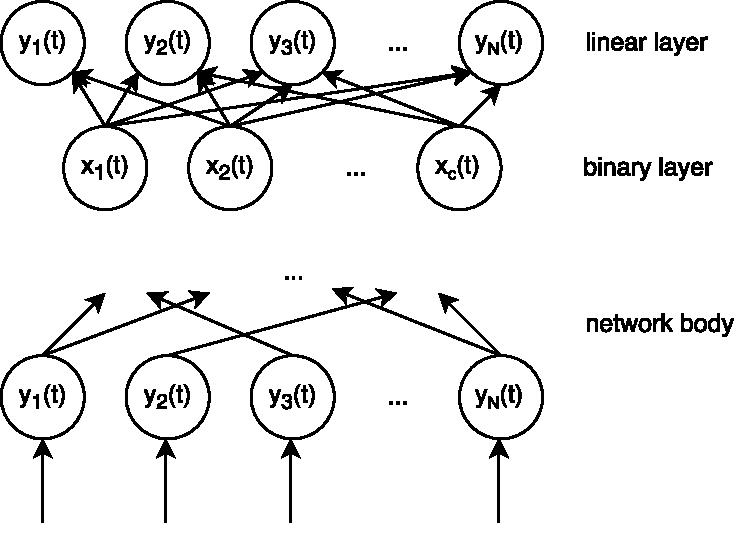
\includegraphics[width=0.75\linewidth]{bolt/neural_net.pdf}
\caption[BOLT: A graphical representation of the neural network used to identify binary additive subcomponents.]{A graphical representation of the neural network used to identify binary additive subcomponents. $x_i(t)$ denote nodes with binary outputs. The activation functions used in the network body are unconstrained.}
\label{fig_sim}
\end{figure}
Unlike existing energy disaggregation approaches that try to disaggregate power, the approach introduced here tries to disaggregate current waveforms. Like power, current is an additive quantity and appliances often exhibit very distinct waveforms. If two appliances are turned on at the same time, the superposition of both appliance waveforms will be measured. In this paper, we show how to recover building blocks of the aggregate current waveforms that contain appliance information using Binary Matrix Factorization as solved by the neural network described above. Every building block or component $i$ is associated with a binary time series ($i$th row of $X$, \emph{when}) and a waveform or loading ($i$th column of $G$, \emph{what}).\\
The neural network that decomposes the aggregate current waveforms into components is trained like an autoencoder, i.e. the desired output is equal to the input but in principle additional information could be incorporated in the input layer that might aide energy disaggregation (e.g., time of the day or outside temperature\footnote{A coffee machine is more likely to be turned on in the morning, a heater is more likely to be turned on when it is cold outside.}). The topology of the network is constrained in such a way that the network has to piece the aggregate current waveforms together using a limited number of additive components. This is achieved by using a linear activation in the output layer and a binary activation in the one but last layer. Figure \ref{fig_sim} shows a graphical depiction of such a network.\\
The stream of current measurements is sliced according to zero-crossings detected in the voltage signal. This results in a matrix $Y \in \mathbb{R}^{N \times T}$ with $T$ being the number of detected cycles and $N$ the number of samples within one cycle (i.e. 200 for a sampling rate of 12kHz and a line frequency of 60Hz). Let $y(t)$ with $t \in [0,T]$ be the current measured within cycle $t$ (i.e., the $t$-th column of $Y$). Let $x(t) \in \{0,1\}^c$ be the activation of the binary layer given the input $y(t) \in \mathbb{R}^{N}$ and $G \in R^{c \times N}$ be the weights connecting the binary and output layer. \\
The network is fed the aggregate current waveforms as a vector of size $N$ containing both the real and imaginary parts of the Fast Fourier Transform (FFT) of $y(t)$. Since the active power consumed by an appliance cannot be negative and most of the power is consumed at line frequency, $G$ is constrained in such a way that the column representing the line frequency (60Hz in the U.S. and 50Hz in Europe) must be non-negative. Note that enforcing this constraint in time-domain is non-trivial.\\
The model is trained in a fully unsupervised way: given the aggregate waveforms, the network is trained to reconstruct them using a limited number of additive building blocks which are assumed to constitute (sub-)appliance waveforms.\\
In order to minimize its training error, the network is forced to activate some of its binary units and adjust the binary-linear weights in such a way that it can capture most of the variability of the aggregate signal. That means, the network must find a set of reoccurring patterns in the aggregate waveforms and for every aggregate waveform, the network must activate a subset of these patterns whose sum best explains the aggregate waveform. In other words, the network finds appropriate values for $X$ and $G$, which minimize $||XG - Y||$.\\
The binary units in the one-but-last layer cause the network's output to be non-smooth, i.e. if the input is slightly perturbed, an additional binary unit might become active or deactivate, thus causing a sudden jump or drop in the output. This is actually a desirable characteristic of the network since the aggregate power trace is also highly non-smooth, i.e. if an appliance is turned on or off, the aggregate power will also jump or drop according to the power consumption of the appliance. The non-smoothness however causes gradients to be ill-defined. \\
 The activation of the binary units is defined as: 
\begin{equation*}
f_b(x)=
\begin{cases}
1 & \text{if } x > 0\\
0 & \text{else}
\end{cases}
\end{equation*}
The derivative of $f_b$ is always $0$ except for $x = 0$ where it is not defined. 
The binary activation can also be understood as 
\begin{align*}
f_b(x) &= \lim_{a \rightarrow \infty} \frac{1}{1 + e^{-ax}}\\
\end{align*}
Let $s(x) = (1 + e^{-ax})^{-1}$.  The derivative of $s(x)$ asymptotically tends to $0$ for $\lim_{x \rightarrow \pm \infty}$ and the bigger $a$, the faster $s(x)$ becomes practically $0$ for digital computing purposes. In order to avoid \emph{vanishing gradients}, the gradient of $f_b(x)$ is set to $\frac{d s(x)}{dx}$ with $a = 1$. This is similar to rounding the outputs in the forward pass and using the actual values for backpropagation.\\
The activations of the hidden units in layers lower than the one-but-last are unconstrained. In principle any activation can be used but, in this work, a leaky rectifying linear unit is employed whose activation is: $f_r(x) = max(ax, x)$. The body of the network (all layers up until the binary layer) has to approximate an NP-complete problem, whereas the linear output units perform a simple linear regression. That means that we choose a computationally powerful body, i.e. many layers and units\footnote{To illustrate this point, in our experiments we noticed that adding a single non-linear layer before the binary layer decreases the training error 5-fold.}. 


\section{Subcomponent identification}
The neural network described was used to identify additive subcomponents in the BLUED \cite{anderson2012blued} dataset. BLUED was collected at a residential building in Pittsburgh, PA, USA during October 2011 with a sampling frequency of 12kHz. In order to preserve phase information of the current signal, zero-crossing which signify the beginning and end of cycles were detected in the voltage signal. Voltage-aligned current measurements spanning 60 consecutive cycles (\~{}1 second) were extracted, i.e. sequences of 12000 data points aligned with the detected zero-crossing. The real and imaginary parts of the first 2400 values of the FFT of the 12000 data points were concatenated into a matrix $Y \in \mathbb{R}^{T \times 4800}$ resulting in an effective sampling rate of 4.8kHz with $T$ being the length of the dataset in seconds (in this case 440000). A 3-layer neural network created with keras\footnote{http://keras.io} was used to perform the binary matrix factorization described earlier. The input layer consists of 3000 leaky rectifying units ($a = 0.5$) that project the input down onto a layer with 2000 leaky rectifying units, which in turn output onto 100 binary hidden units. Thus, the aggregate current waveforms are assumed to be composed from 100 additive building blocks.\\
\begin{figure}[!ht]
\begin{tabular}{cc}
  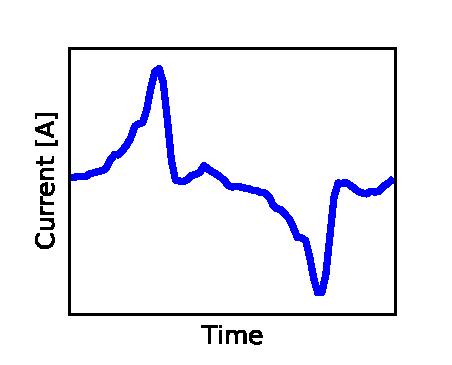
\includegraphics[width=0.45\linewidth]{bolt/comp_all18.eps} &   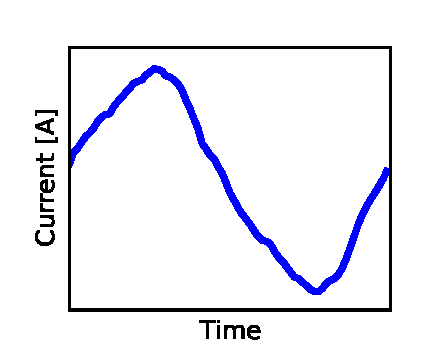
\includegraphics[width=0.45\linewidth]{bolt/comp_all78.eps} \\
(a) & (b) \\
 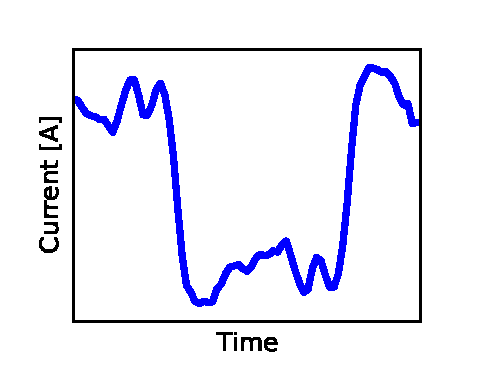
\includegraphics[width=0.45\linewidth]{bolt/comp_all1.eps} &   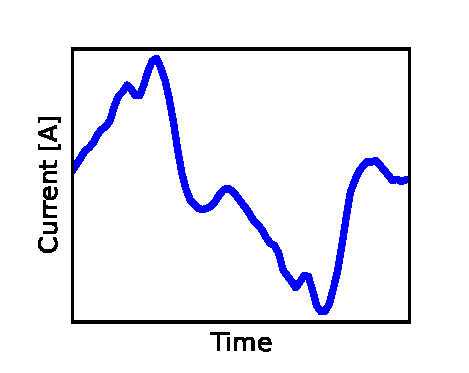
\includegraphics[width=0.45\linewidth]{bolt/comp_all26.eps} \\
(c)  & (d) \\
\end{tabular}
\caption[BOLT: Example inferred subcomponents extracted with BOLT.]{Four out of the 100 inferred subcomponents in the aggregate signal: (a) waveform of a power supply for a computer, (b) an almost purely resistive load, (c) highly reactive load, and (d) superposition of appliances}
\label{fg:wv}
\end{figure}

The weights between a binary unit and the linear output units (i.e., the columns of $G$) incorporate the information about the waveform of the corresponding component. Figure \ref{fg:wv} shows some of the inferred subcomponents identified in the aggregate signal after transforming them back into time-domain. Figure \ref{fg:wv} a) shows a waveform whose temporal activity is highly correlated with the activity of a computer. Computers like many other electronics are powered by a power supply unit (PSU) which transforms AC to DC current by rectification. The inferred waveform shows how the rectifier consumes power when the voltage peaks. We can also infer that the computer's PSU performs full-wave rectification as opposed to half-wave rectification in which case only single peak would be shown.\\

Figure \ref{fg:wv}b shows a generic sinusoidal waveform. Unfortunately, this waveform cannot easily be attributed to any specific appliance. In the experiment conducted on the BLUED dataset, the network infers 12 highly sinusoidal components, and for none of these their corresponding $X$ row correlates highly with any single appliance ground truth. This is most likely due to the fact that the network can use purely sinusoidal components as building blocks for purely resistive loads. For example, if there are two purely resistive loads consuming 200W and 250W respectively, the network has multiple equally valid solutions for decomposing their waveforms. In a perfect world, the network would allot one component to be a 200W sinusoidal and the other to be a 250W sinusoidal. This would readily disaggregate the energy of both appliances. However, the network could also explain the aggregate waveform by inferring one 200W sinusoidal and another 50W sinusoidal in which case non-linear re-aggregation of the inferred subcomponents is required to disaggregate the appliances.\\

Figure \ref{fg:wv} c) shows a component consuming solely reactive power. With very few exceptions, this component is almost always active during the whole duration of the dataset. The component does not consume any active power.\\

Figure \ref{fg:wv} d) shows a component with two peaks. The inferred component shows similarly high temporal correlation with the laptop and the desk lamp which suggests that the inferred component might be the superposition of those two appliances. The algorithm does not guarantee that the waveform of every inferred subcomponent is caused by a single appliance.

\begin{figure}
\begin{tabularx}{\textwidth}{XcXcX}
\noindent\parbox[c]{\hsize}{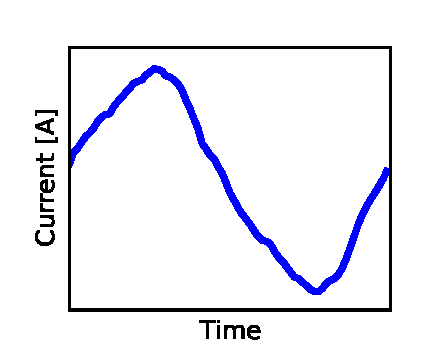
\includegraphics[width=0.75\linewidth]{bolt/comp_all78.eps}}  &+&  \noindent\parbox[c]{\hsize}{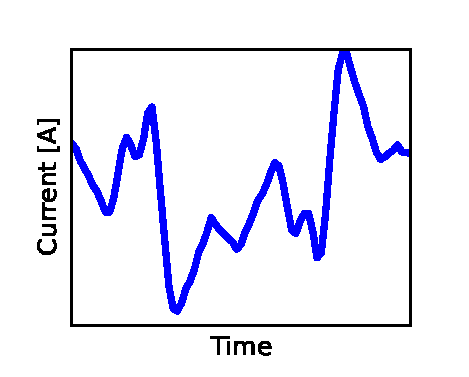
\includegraphics[width=0.75\linewidth]{bolt/comp_all5.eps}}   &=&  \noindent\parbox[c]{\hsize}{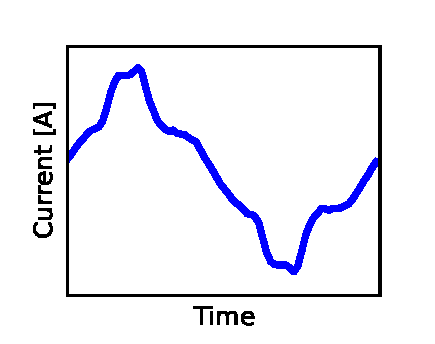
\includegraphics[width=0.75\linewidth]{bolt/sum70_5.eps}}
\end{tabularx}
\caption[BOLT: The sum of a seemingly noisy and a sinusoidal component.]{The sum of a seemingly noisy and a sinusoidal component.}
\label{fg:wv_sum}
\end{figure}

Figure \ref{fg:wv_sum} shows a seemingly noisy component. Even though the network is constrained in such a way that the power at line frequency must be greater than zero, the component exhibits negative power overall (assuming stable voltage at 110V), i.e. the component alone cannot represent an appliance. However, if this component is added to a sinusoid, the resulting component shows much structure and is similar to other inferred components. The seemingly noisy component can modify other components whose structure it can partially hijack. %The 'noisy component' could also be an indicator for a multi-state device whose waveform scales up with power consumption since it can take an arbitrary resistive load and shift its shape.\footnote{We are unable to verify this claim so far}\\

To sum up, the inferred subcomponents seem to be either: (a) the waveform of a specific appliance, (b) the superposition of the waveforms of multiple appliances, (c) modifier that requires the presence of another subcomponent, (d) a sinusoidal building block; or (e) a duplicate of another subcomponent.

\section{Combining Binary Components}
Following the intuition gained about the nature of the inferred subcomponents, supervised and unsupervised approaches for inferring appliance activity given the activities of inferred subcomponents will be discussed.\\
Let the matrix containing the activations of the inferred subcomponents be $X \in (0,1)^{d \times T}$, with $d$ being the number of components and $T$ the number of current and voltage cycles. The $t$th row of $X$ denotes the hidden states of the network $x(t)$ given input $y(t)$.

\begin{description}
\item[Supervised Re-Aggregation] In the supervised case, we also assume knowledge of a matrix containing ground truth of whether or not a specific appliance is turned on or off at any given voltage cycle. Let $G \in (0,1)^{T \times A}$ denote this matrix with $A$ being the number of appliances.
\item[Logistic Regression] An algorithm is sought that can model a binary response given predictors. Logistic regression can be used to predict the probability of binary probabilistic outcomes. We are interested in modeling $P(g_i (t) = 1 | x(t))$. Using logistic regression to model this distribution assumes that $P(g_i (t) = 1 | x(t))$ is a Bernoulli distribution with
\begin{align*}
P(g_i (t) = 1 | x(t)) = \frac{1}{1+exp[w_i^T x(t)]}
\end{align*}
 The model parameter $w_i$ can be obtained using a maximum likelihood estimate.
\item[Boolean Re-Aggregation] Logistic Regression learns a complex non-linear function but scenarios in which Logistic Regression can be applied without access to ground truth seem unlikely. Collecting ground truth requires sub-metering of appliances and is often prohibitively expensive. An unsupervised approach to re-aggregation will most likely analyze the temporal activity and the shape of the waveform of the inferred subcomponents and then combine subcomponents into appliances.\\
The temporal activity of a subcomponent, i.e. $x_j \in \{0,1\}^T$ (the columns of $X$), can be viewed as a sequence of truth values indicating if the respective component is active. Let $\lor$ be the element-wise $or$-operator such that $x_j \lor x_i \in \{0,1\}^T$. Since the network might infer the same component (according to its waveform) multiple times, a successful re-aggregation strategy would need to identify components with similar waveforms and connect them via the $\lor$-function.\\
Furthermore, imagine a scenario with two purely resistive appliances consuming 200W and 250W. As described earlier, the network could explain the aggregate waveforms by allocating one 200W sinusoid and one 50W sinusoid. Let $x_1$ and $x_2$ be the subcomponents constituting the inferred sinusoidal building blocks respectively. For the temporal activity pattern of the appliance consuming 250W, the following needs to be true: $x_1 \land x_2$, whereas for the appliance consuming 200W, we need to have $x_1 \land \neg  x_2$.\\
In order to provide an upper bound for an unsupervised algorithm that finds a boolean function connecting subcomponents, an algorithm is introduced that performs a greedy search over boolean functions in a supervised way: A function $f(x_j,...,x_k)$ is sought that maximizes the similarity between $g_i$ (the temporal activity of appliance $i$) and the output of that function on a subset of binary components $x_j,... ,x_k$. We furthermore assume that $f$ solely contains the operators $\lor, \land$ and $\neg \land$. As a similarity measure the F1 score is used.\\
The greedy algorithm iteratively adds one component to the function. The algorithm is initialized believing that $g_i$ is always turned on, i.e. $f_0 = (1)^T$. Then it iterates over all $x_i$ and computes the F1 score that would result in either appending $\land x_i$, $\lor x_i$ or $\land \neg x_i$ to $f$. After one sweep, the component that resulted in a maximal increase in F1 score is selected and appended to $f$. This is repeated until the F1 score cannot be improved further.
\end{description}
 
 \section{Unsupervised Re-Aggregation}
 \subsection{Lower bound on unsupervised Re-Aggregation}
 The assumption that every inferred subcomponent readily constitutes an appliance is a far-fetched assumption but can serve as a lower bound for unsupervised re-aggregation strategies. For each appliance, the component resulting in the highest F1 score compared to the ground truth is selected. This assumes that it is possible to classify subcomponent waveforms and their temporal activity patterns in order to infer appliances or receive this information from a user.
 
 \subsection{Na\"ive Re-Aggregation}
 When applying the supervised boolean re-aggregation described earlier, the algorithm seems to favor connecting subcomponents using the $\land$-operator. Following this intuition, a na\"ive re-aggregation strategy is introduced: two similarity metrics are defined: $d_w$ and $d_a$. The purpose of $d_w$ is to measure the similarity between the waveforms of two subcomponents, whereas $d_a$ measures the similarity between the temporal activity patterns of two subcomponents. We assume knowledge of a seed-component which in this case is the component resulting in the highest F1 score when comparing components to the ground truth. So ultimately, the goal is to improve the lower bound on unsupervised re-aggregation introduced earlier.\\
 For every appliance the seed-component is found using the ground truth. Let $x_{a,s}$ be the seed-component of appliances $a$. Then, for every component, a weighted sum of the similarity scores is computed: $d(x_{a,s}, x_i) = \lambda d_w(x_{a,s}, x_i) + (1-\lambda) d_a(x_{a,s}, x_i)$. Let $X_d$ be the set of components for which this similarity is bigger than a threshold $\epsilon$, i.e. $X_d(a) = \{x_i | d(x_{a,s}, x_i) > \epsilon\}$. All components in $X_d(a)$ are connected using the $\land$-operator, i.e. $\hat{g}_a = \bigwedge_{x_i \in X_d(a)} x_i$.
 
 \section{Results}
 \subsection{Supervised}
 In the supervised scenario, the power trace of the individual appliances can be estimated in a straight forward way if we assume that the $on$ and $off$ consumptions of appliances are known. Let $\hat{g}_a$ be the boolean time series representing the estimate for appliance $a$, then $\hat{p} = p_{on} \hat{g}_a  + p_{off}(1-\hat{g}_a)$. As a measurement of the goodness of the inferred power trace, the mean deviation error is employed: \begin{align*}
E(p, \hat{p}) = \sum_{i,t} \frac{|p_i(t) - \hat{p}_i(t)|}{p_i(t)}
\end{align*}

BOLT poses energy disaggregation as a waveform classification problem. Current waveforms are highly non-iid (independently and identically distributed), which poses a challenge for properly evaluating the performance. Thus, we evaluate the performance in two ways: first, we assume the current readings are iid and therefore randomly split matrix $X$ into a training and test set (50/50 split) for the logistic regression. This might, however, overestimate the performance in some cases but allows us to obtain disaggregation results for every appliance. Second, we perform \emph{snippet cross-validation}. For this, the ground truth is sliced into non-overlapping snippets that contain a single run-cycle of an appliance, i.e. the data is separated between an \emph{off} and an \emph{on}-transition such that every snippet contains a run-cycle and some examples where the appliance is off to ensure that no data is lost. The logistic regression is then trained on all but one snippet and evaluated on the snippet that it was not trained on. Note that such an evaluation is not possible for all appliances (e.g. those appliances that only contain a single run-cycle).
Table \ref{bolt:results} shows the results on the individual appliances for which ground truth data was available. The column ``active'' shows the proportion at which the appliance is active. Since the energy was estimated assuming 2-state appliances, \emph{mean disaggregation error} captures the variance of the appliances to some degree. A perfect 2-state prediction of an appliance with higher variance will always lead to a higher \emph{mean disaggregation error}, even though the energy in sliding windows (or power at a lower temporal resolution) would be predicted perfectly. The lower bound for assuming 2-state appliances and a perfect prediction is shown in the column $E(p)$. $E(\hat{p})$ and $E_S(\hat{p})$ shows the mean disaggregation error using iid- and snippet-evaluation, respectively.\\
Whether or not the algorithm can detect if an appliance is turned on or off was measured using the F1 score (0 - worst, 1 - best). As expected, for iid-evaluation, combining binary subcomponents using logistic regression ($F1_{L}$) outperforms the approach based on greedy search ($F1_{B}$). $F1_{S}$ shows the performance using snippet evaluation.\\
\begin{table}[]
\setlength{\tabcolsep}{1pt}
\centering
\begin{tabular}{l|c|c|c|c|c || c | c}
\hline
Appliance      & Active            & $F1_{B}$ & $F1_{L}$ & E($\hat{p}$) & E($p$) & $F1_{S}$ & $E_s(\hat{p})$ \\ \hline
A/V LR         & 60\%              & 0.89        & 0.98       & 0.04      & 0.009  & - & -\\
Computer 1     & 27.3\%            & 0.88        & 0.99       & 0.05      & 0.042 & 0.96 & 0.10  \\
Desk Lamp      & 21.4\%            & 0.84        & 0.95       & 0.06      & 0.013 & 0.81 & 0.38  \\
DVR            & 20.7\%            & 0.94          & 0.99       & 0.006      & 0.005 & 0.89 & 0.05  \\
Socket LR      & $>0.1\%$ & 0.96        & 0.92       & 0.09      & 0.089 & - & -  \\
Garage Door    & 0.4 \%            & 0.49          & 0.89       & 0.07      & 0.063 & - & -  \\
Iron           & 0.1 \%            & 0.74        & 0.92       & 0.12      & 0.115 & - & -   \\
Laptop 1       & 33.3\%            & 0.75        & 0.92       & 0.34      & 0.272 & - & -  \\
LCD Monitor    & 16.2\%            & 0.73        & 0.94       & 0.12      & 0.029 & 0.79 & 0.38  \\
Monitor 2      & 17.3\%            & 0.80        & 0.92       & 0.20      & 0.089 & - & -   \\
Printer        & 0.1\%             & 0.45           & 0.70       & 0.05      & 0.045 & - & -  \\
Tall Desk Lamp & 21.4\%            & 0.84        & 0.95       & 0.06      & 0.008 & 0.80 & 0.38  \\
TV Basement    & 20.7\%            & 0.94        & 0.99       & 0.05      & 0.029 & 0.88 & 0.26 \\ \hline
Random         & 30\%              & 0           & 0          & -         & -    & 0  & -   \\ \hline \hline
Overall        &                   &             &            & 0.058      & 0.037 & - & 0.18
\end{tabular}
\caption[BOLT: Supervised performance comparison]{``Active'' denotes the proportion during which the appliance was active, $F1_{B}$ and $F1_{L}$ show the performance of the Boolean Search and logistic regression in the iid-evaluation setting whereas $F1_{S}$ shows the performance of the logistic regression using snippet crossvalidation, $E(\hat{p})$ and $E(p)$ show mean disaggregation error of the inferred power trace (Logit) and the lower bound assuming 2-state appliances. $E_S(\hat{p})$ shows the same error using snippet crossvalidation. }
\label{bolt:results}
\end{table}


\begin{table}[]
\setlength{\tabcolsep}{3pt}
\centering
\begin{tabular}{lcc}
\hline
AV-LR  \\
 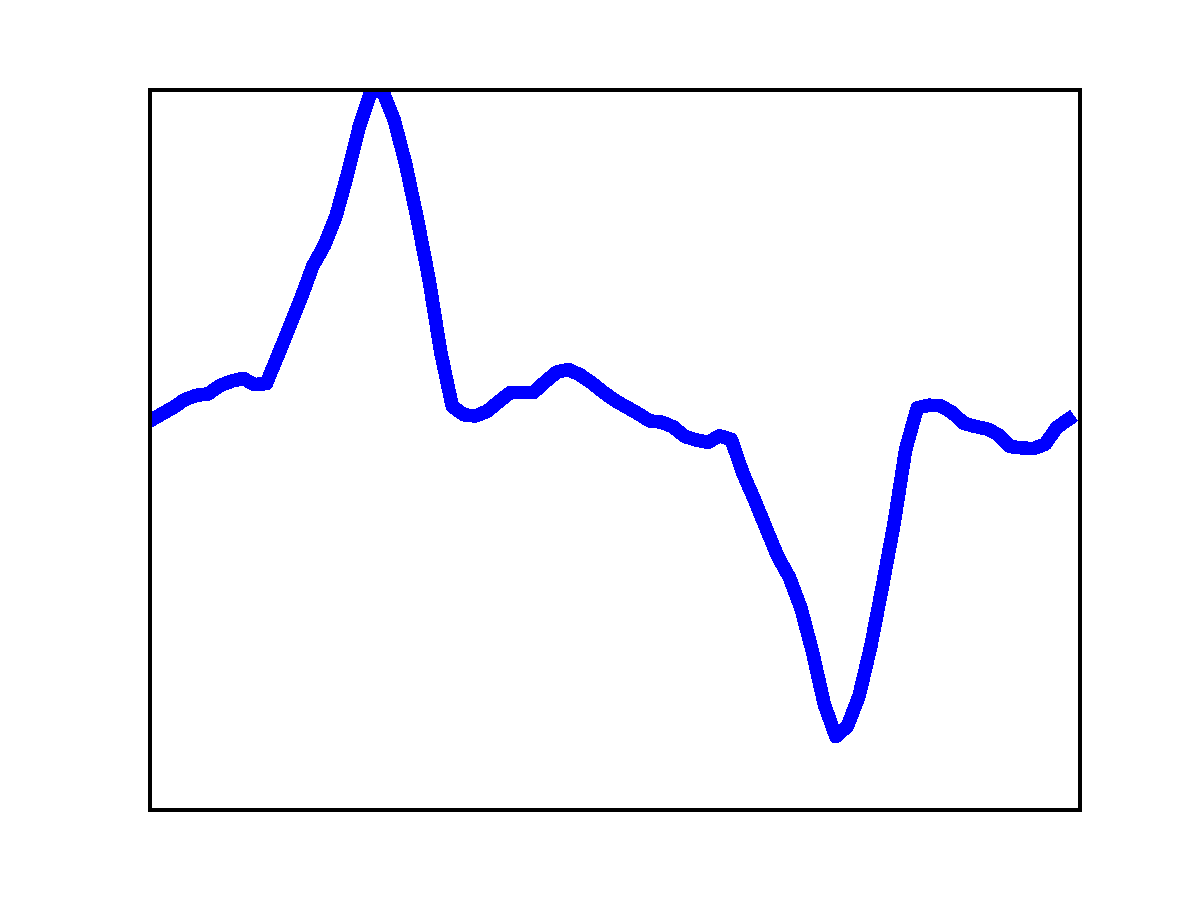
\includegraphics[width=20mm]{comps/comp_all63.pdf}        & 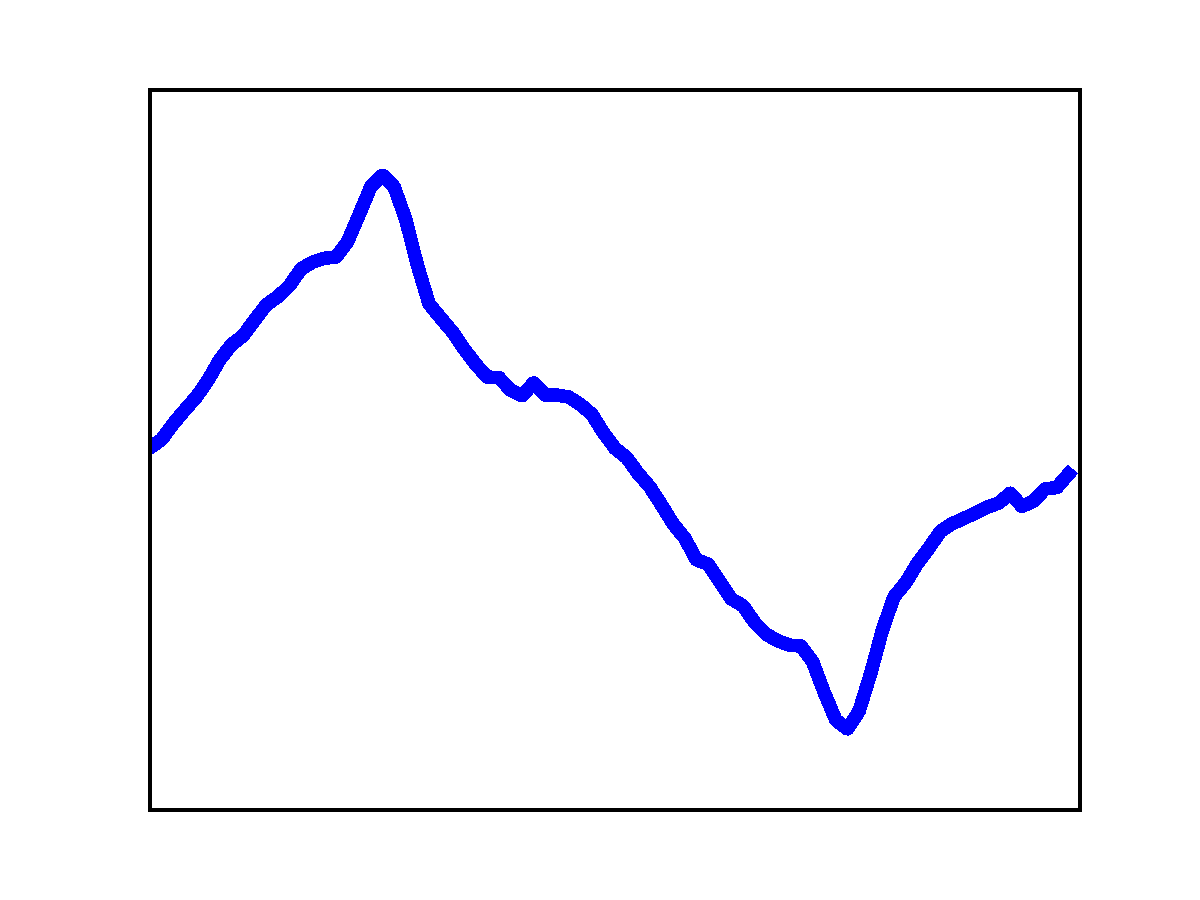
\includegraphics[width=20mm]{comps/comp_all49.pdf}       & 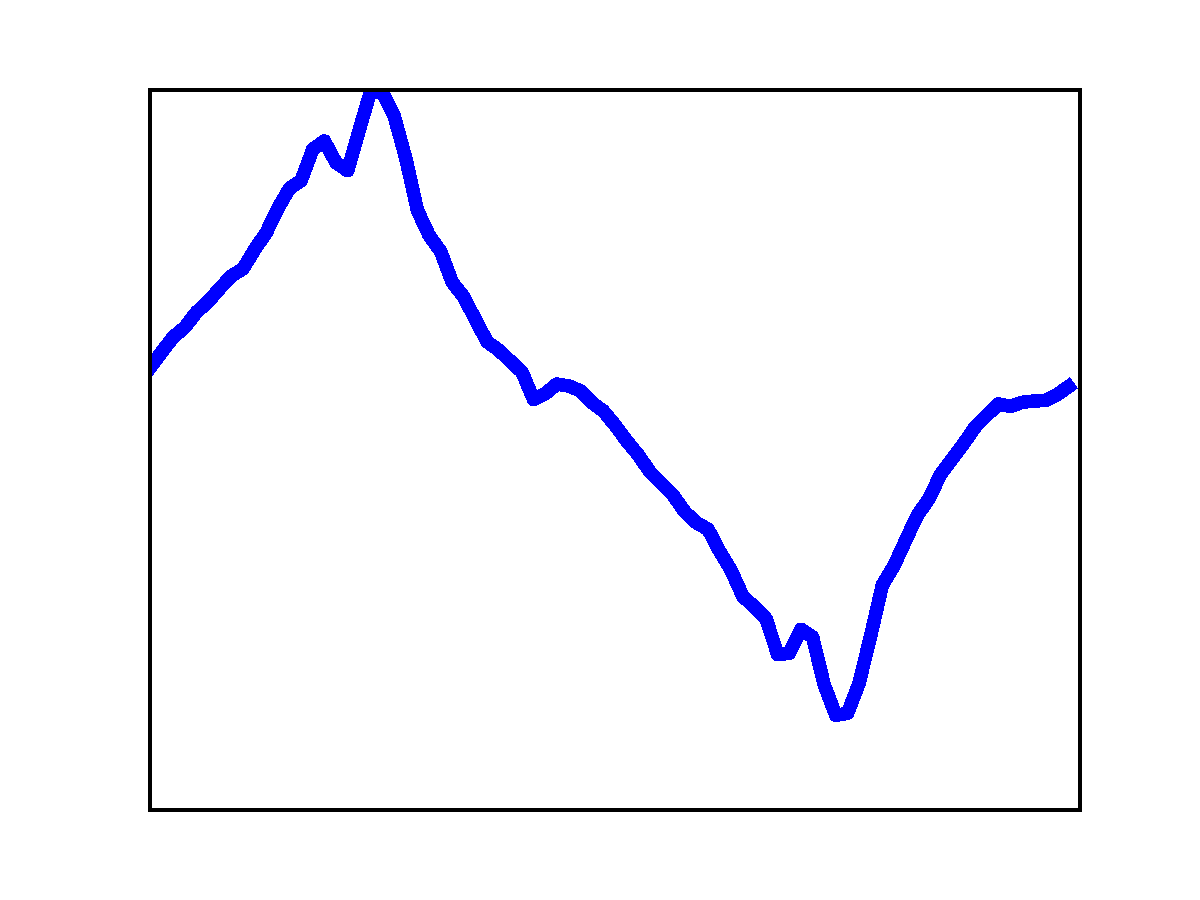
\includegraphics[width=20mm]{comps/comp_all23.pdf}   \\ \hline
Computer 1     \\
 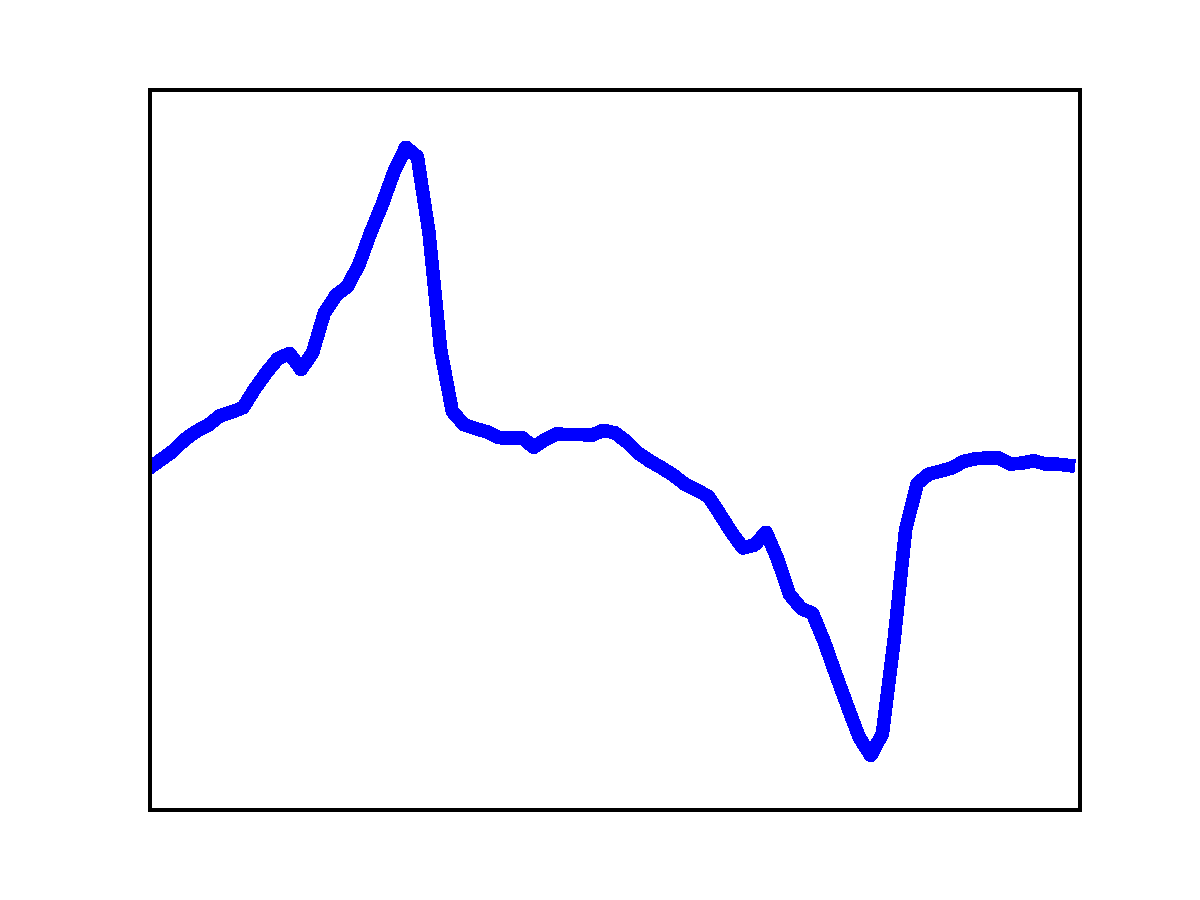
\includegraphics[width=20mm]{comps/comp_all30.pdf}        & 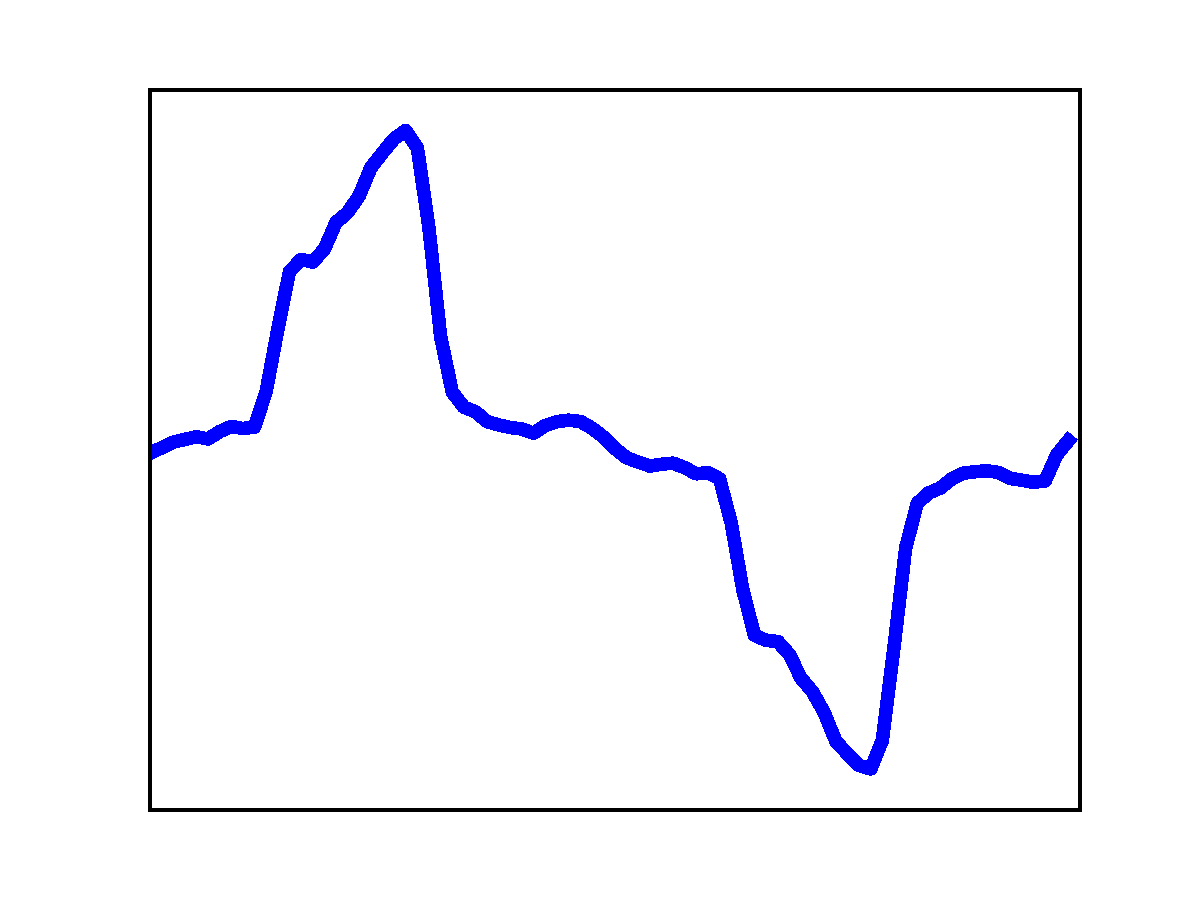
\includegraphics[width=20mm]{comps/comp_all60.pdf}       & 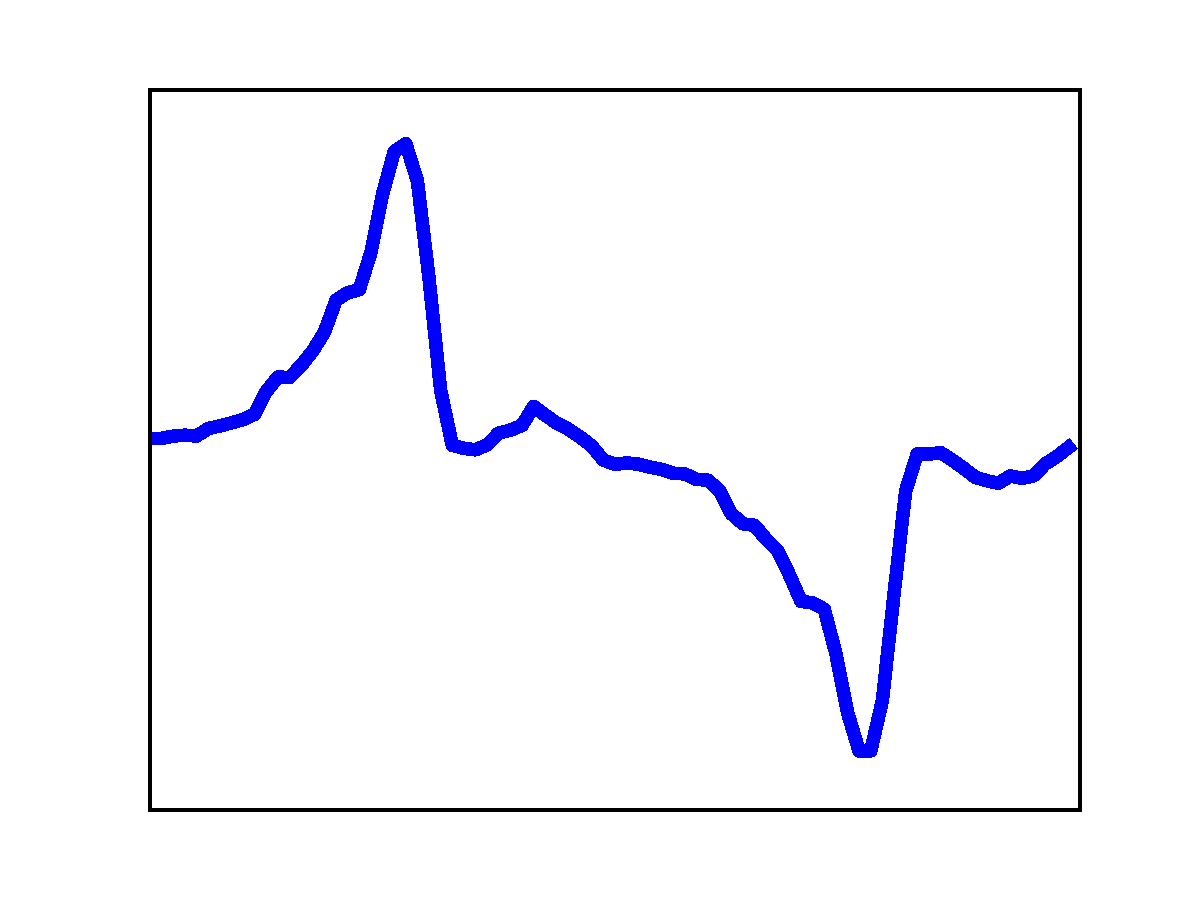
\includegraphics[width=20mm]{comps/comp_all18.pdf}   \\ \hline
DVR            \\
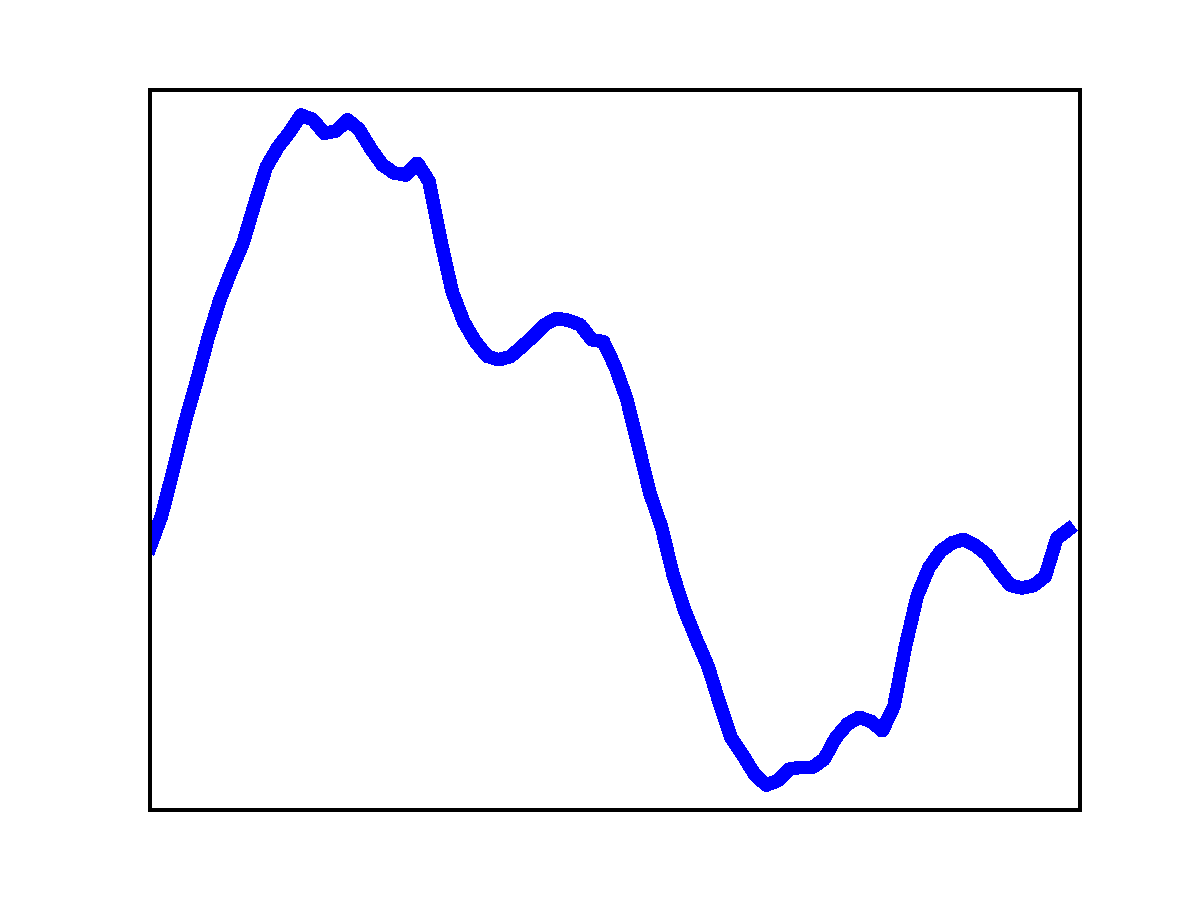
\includegraphics[width=20mm]{comps/comp_all34.pdf}        & 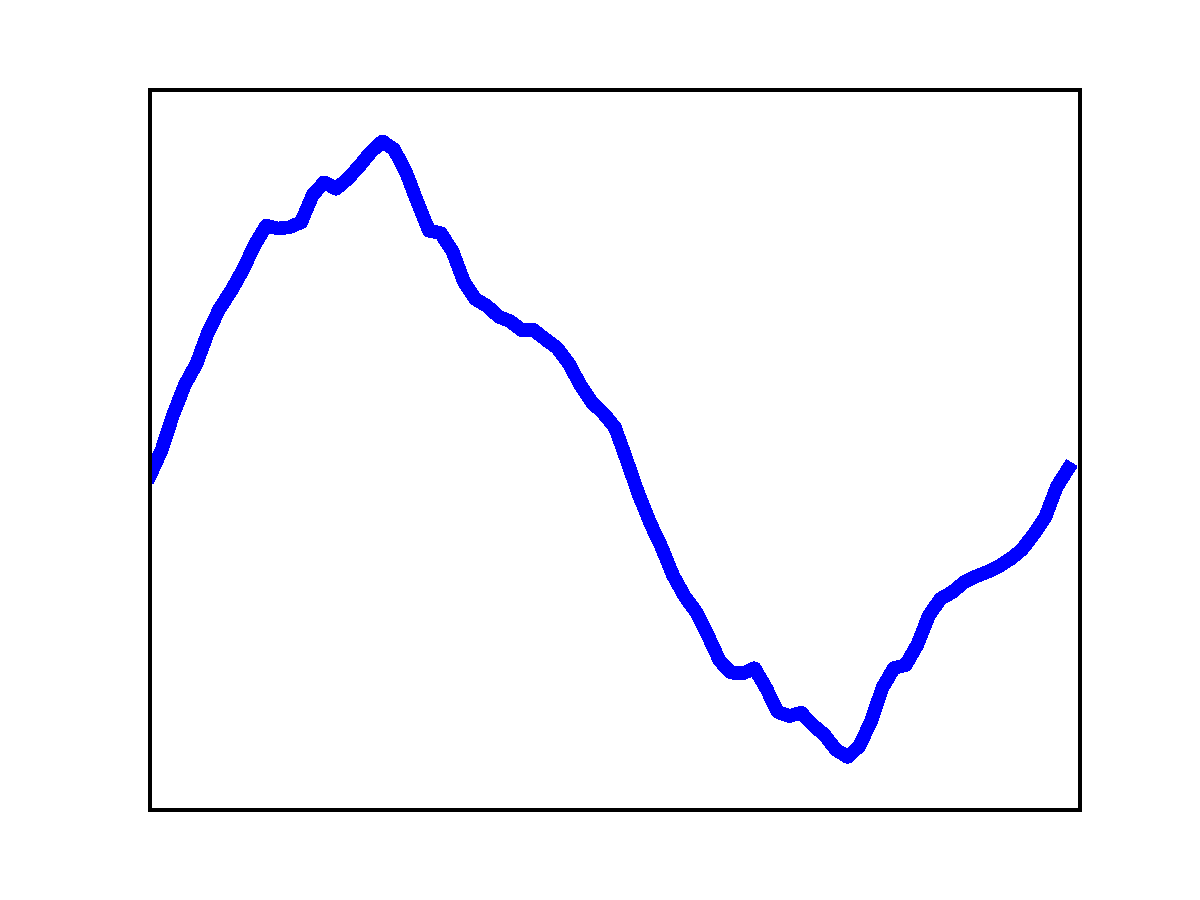
\includegraphics[width=20mm]{comps/comp_all82.pdf}       & 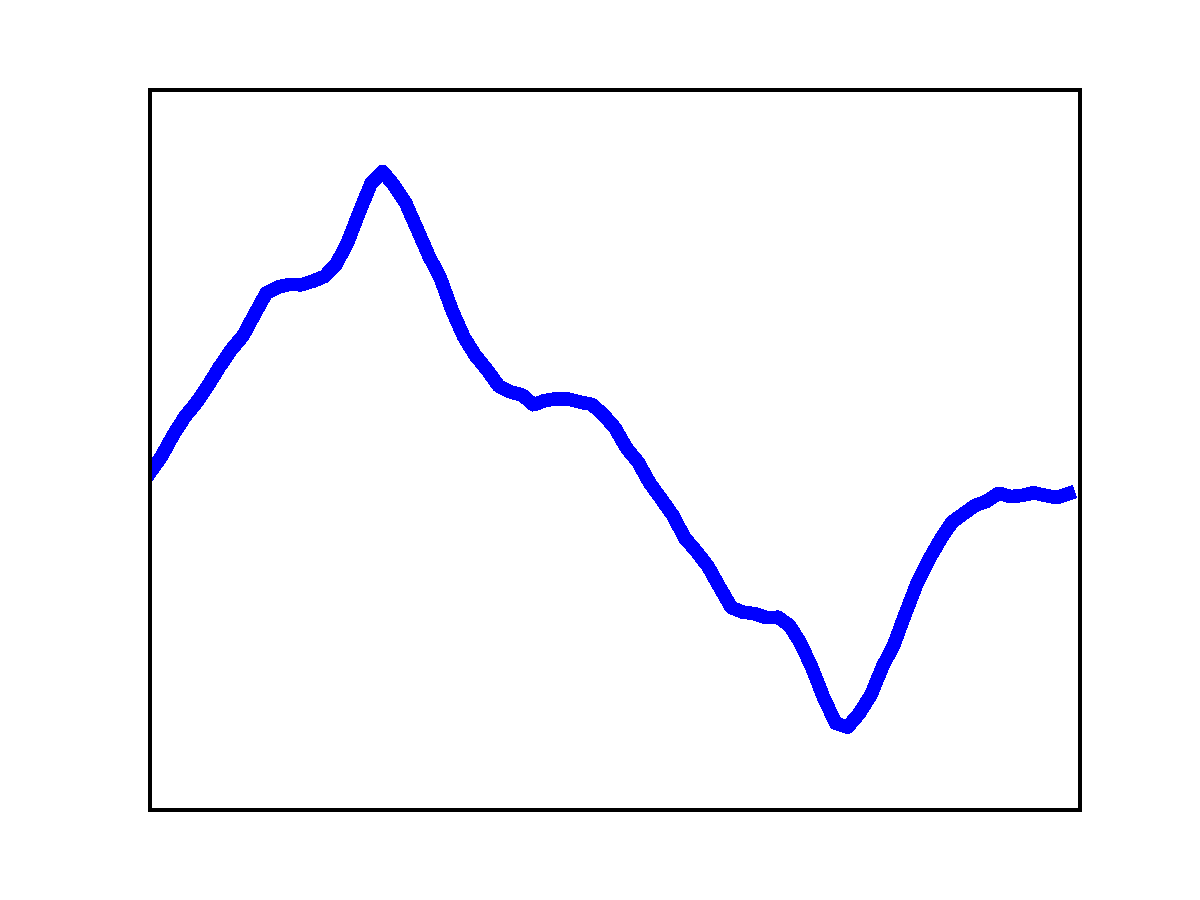
\includegraphics[width=20mm]{comps/comp_all47.pdf}   \\ \hline

Laptop 1     \\
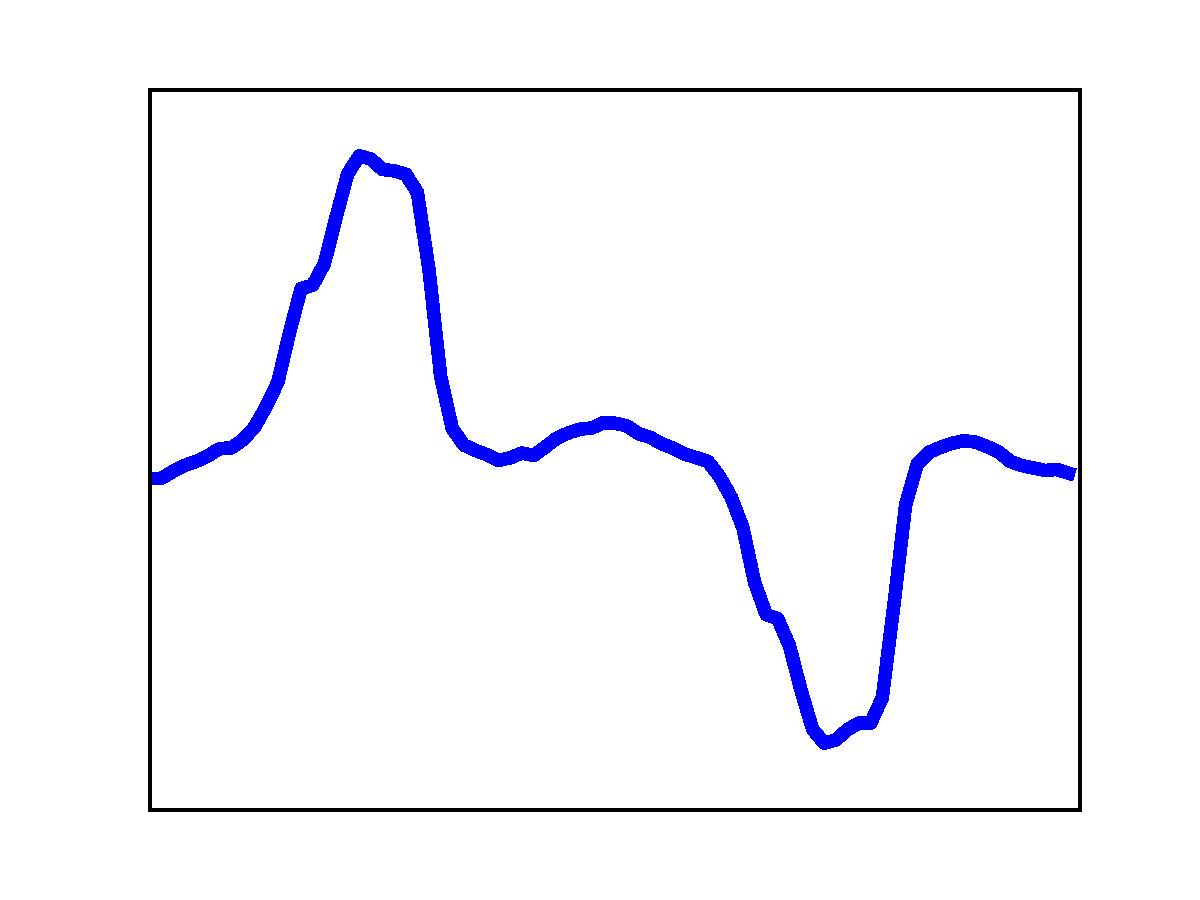
\includegraphics[width=20mm]{comps/comp_all36.pdf}        & 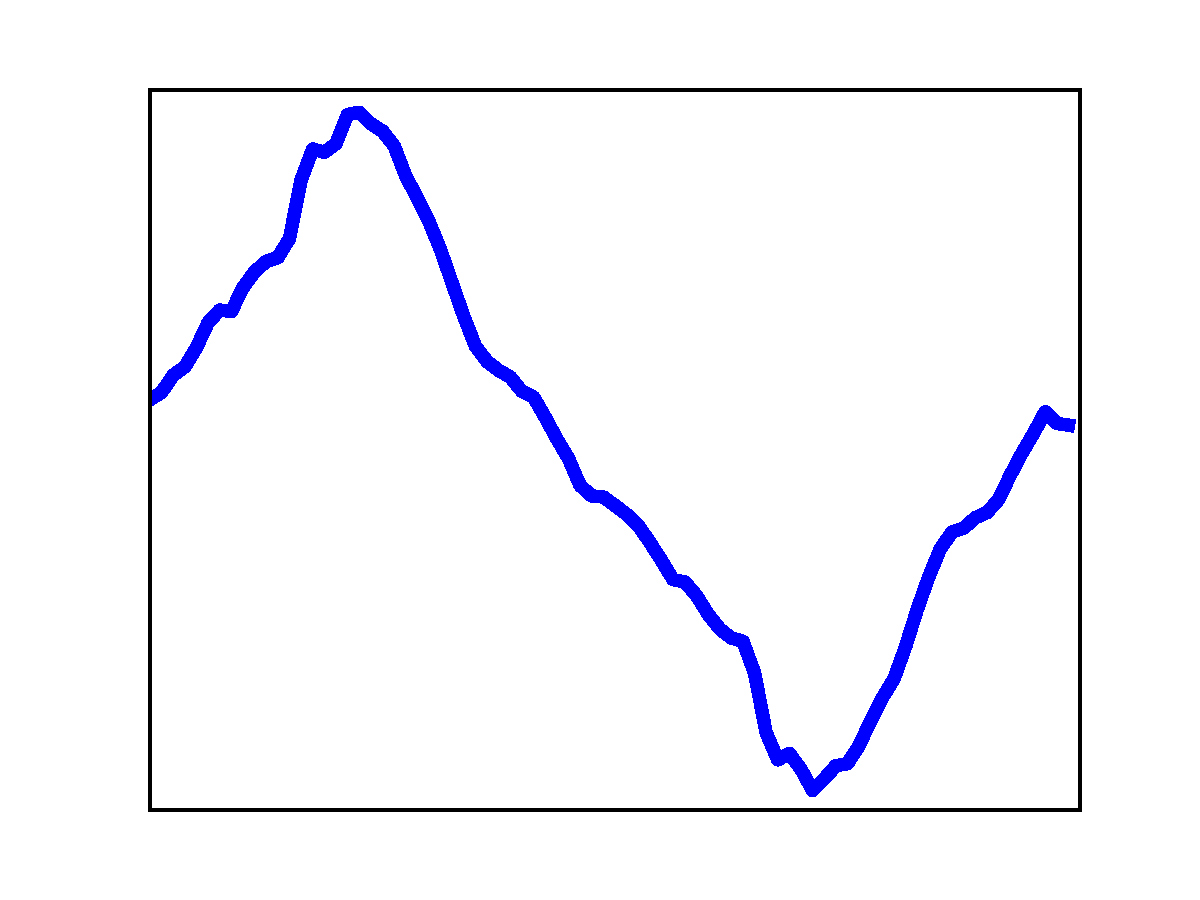
\includegraphics[width=20mm]{comps/comp_all69.pdf}       & 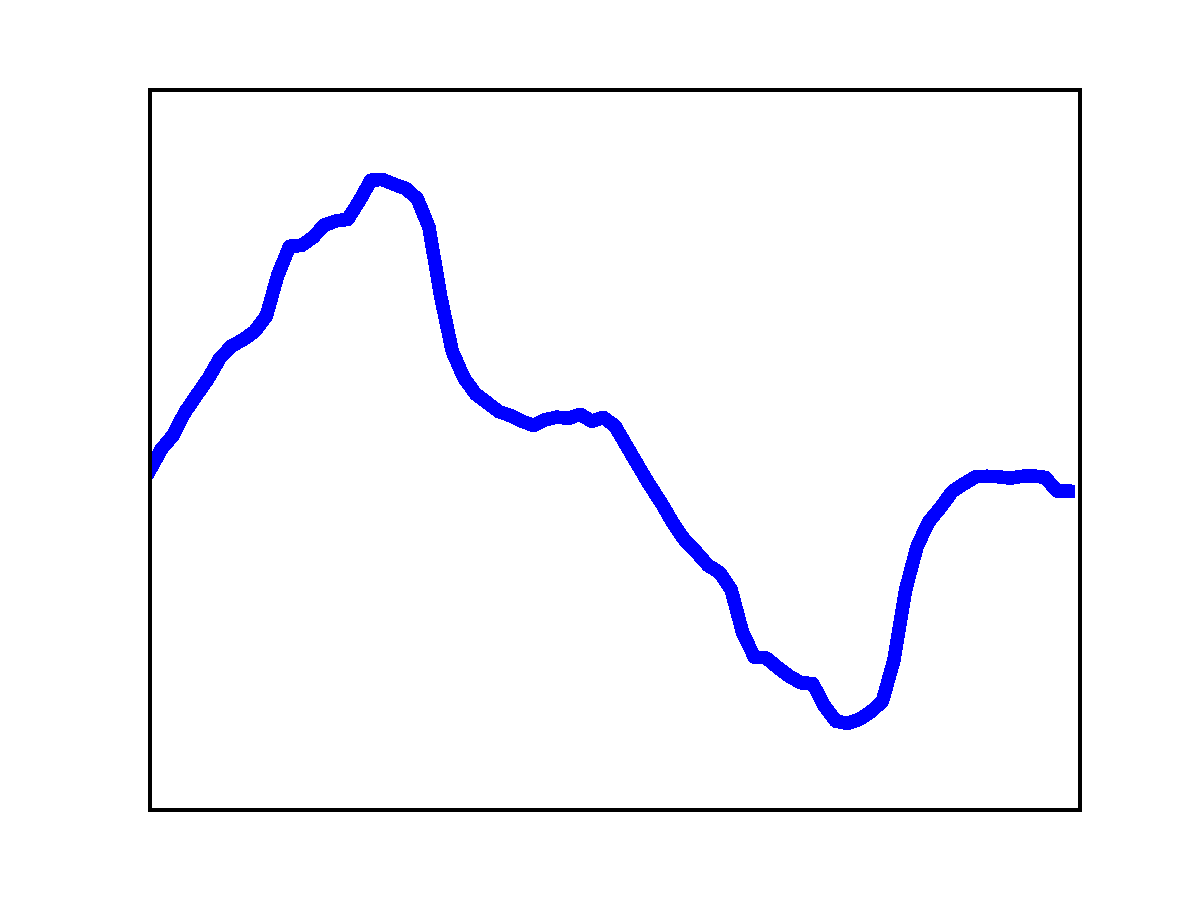
\includegraphics[width=20mm]{comps/comp_all90.pdf}   \\ \hline

LCD Monitor  \\
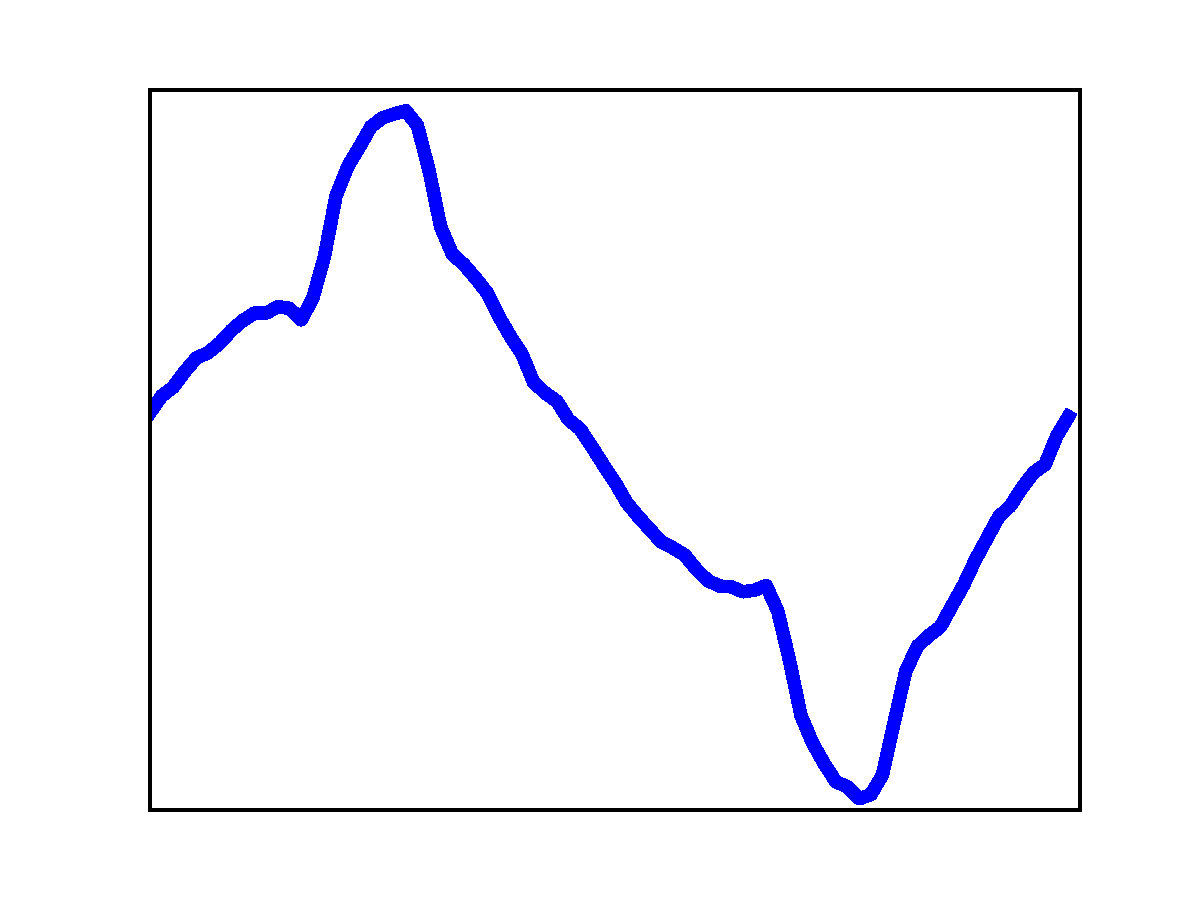
\includegraphics[width=20mm]{comps/comp_all81.pdf}        & 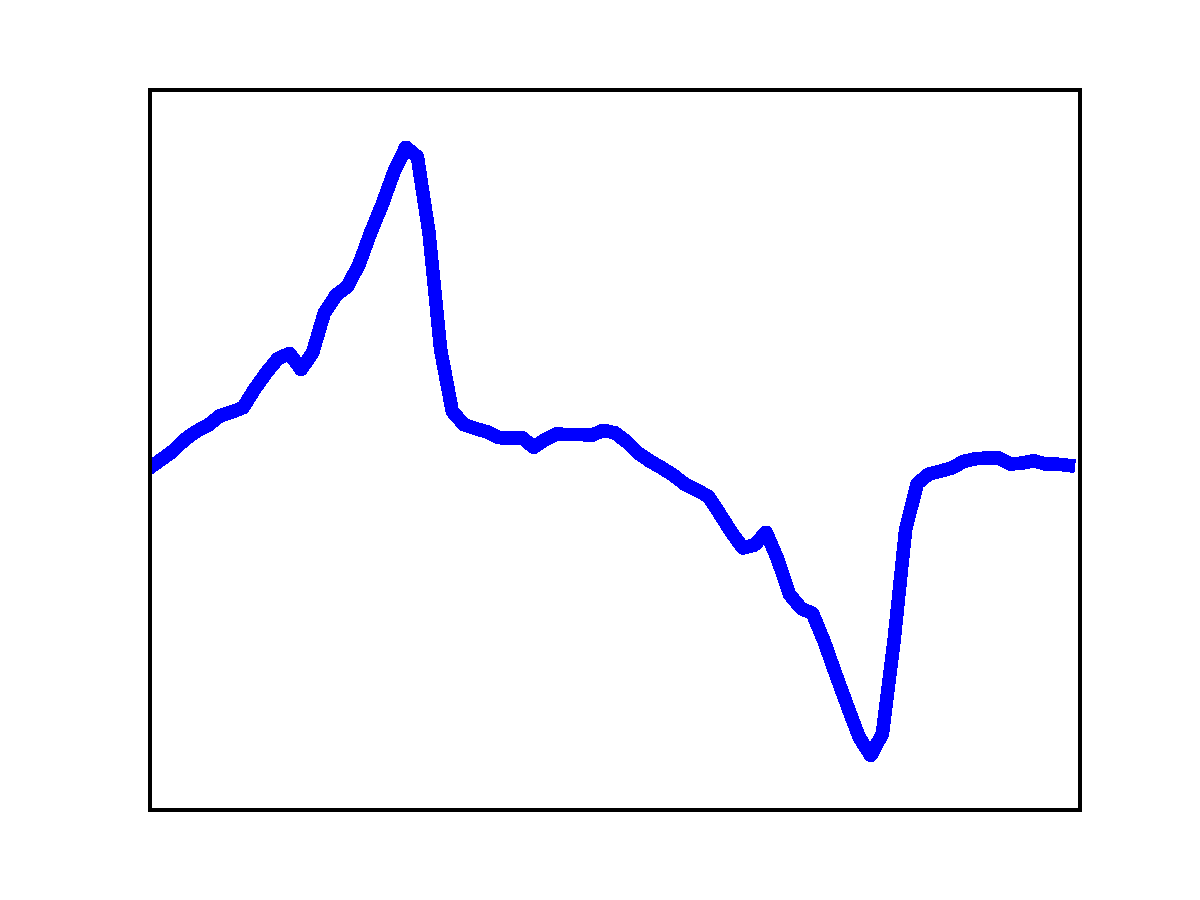
\includegraphics[width=20mm]{comps/comp_all30.pdf}       & 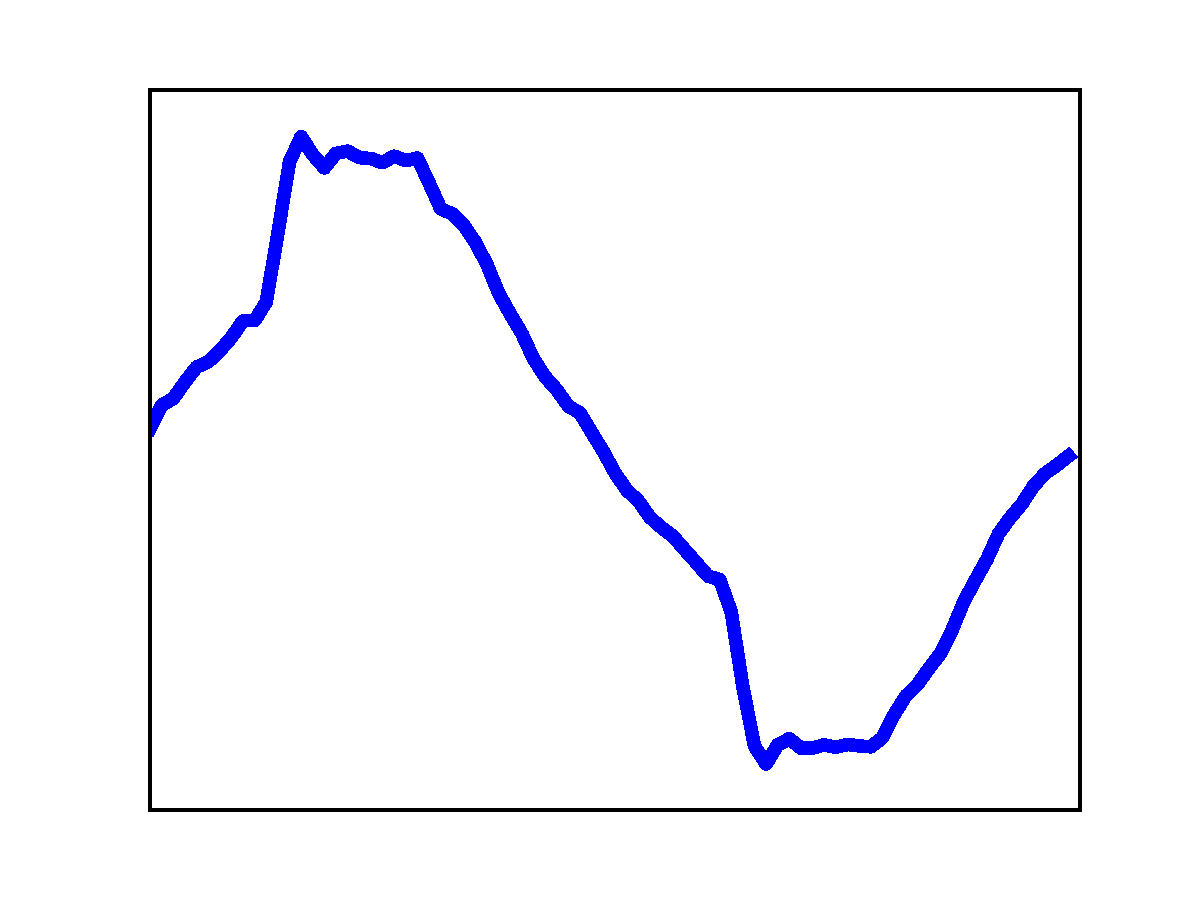
\includegraphics[width=20mm]{comps/comp_all55.pdf}   \\ \hline
Monitor 2      \\
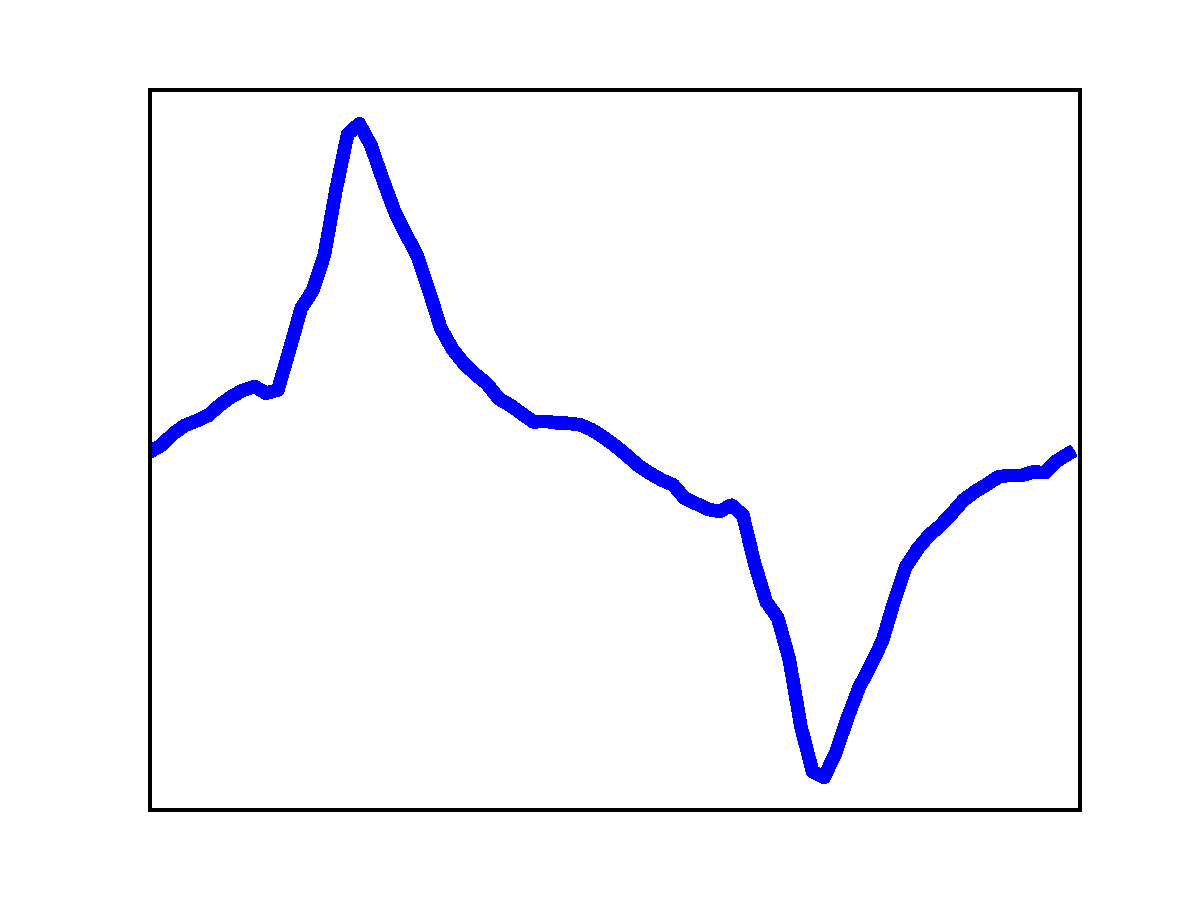
\includegraphics[width=20mm]{comps/comp_all97.pdf}        & 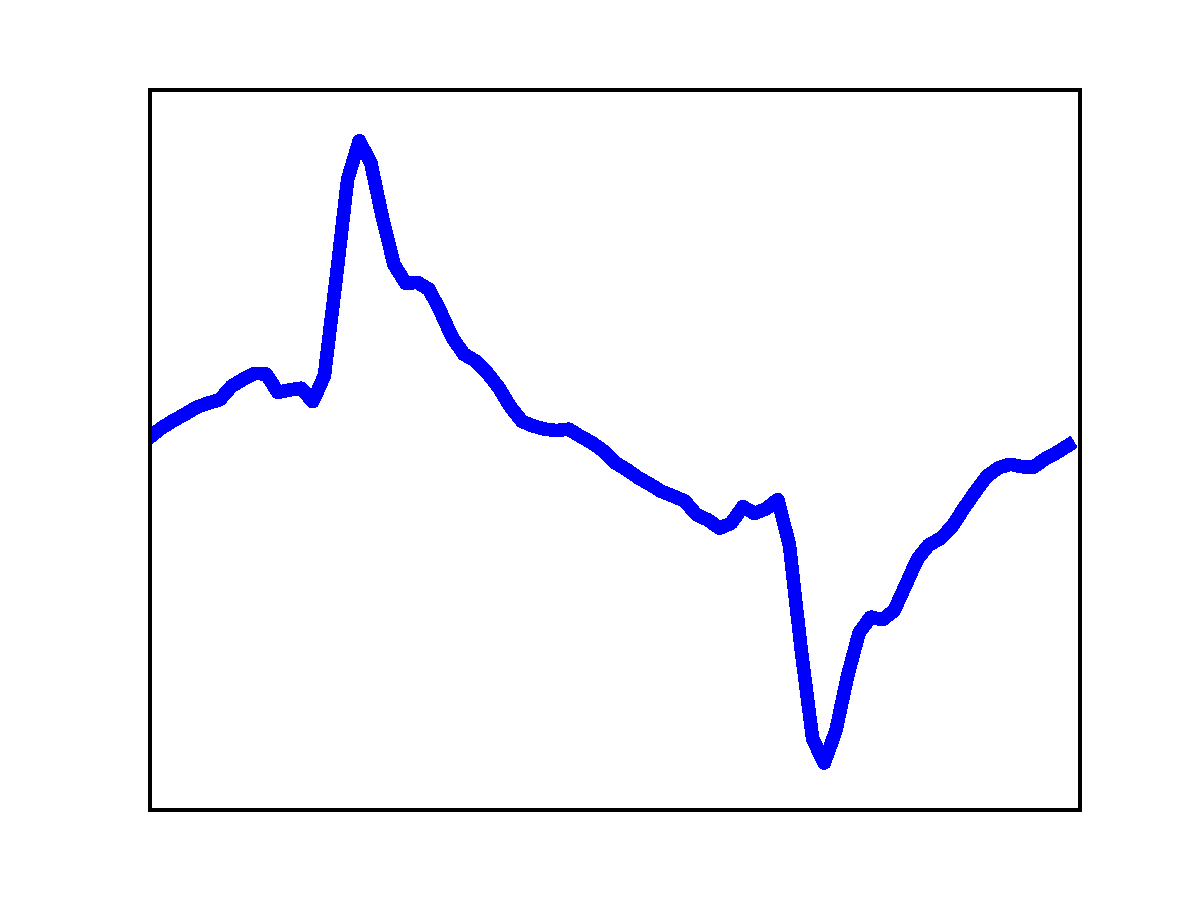
\includegraphics[width=20mm]{comps/comp_all13.pdf}       & 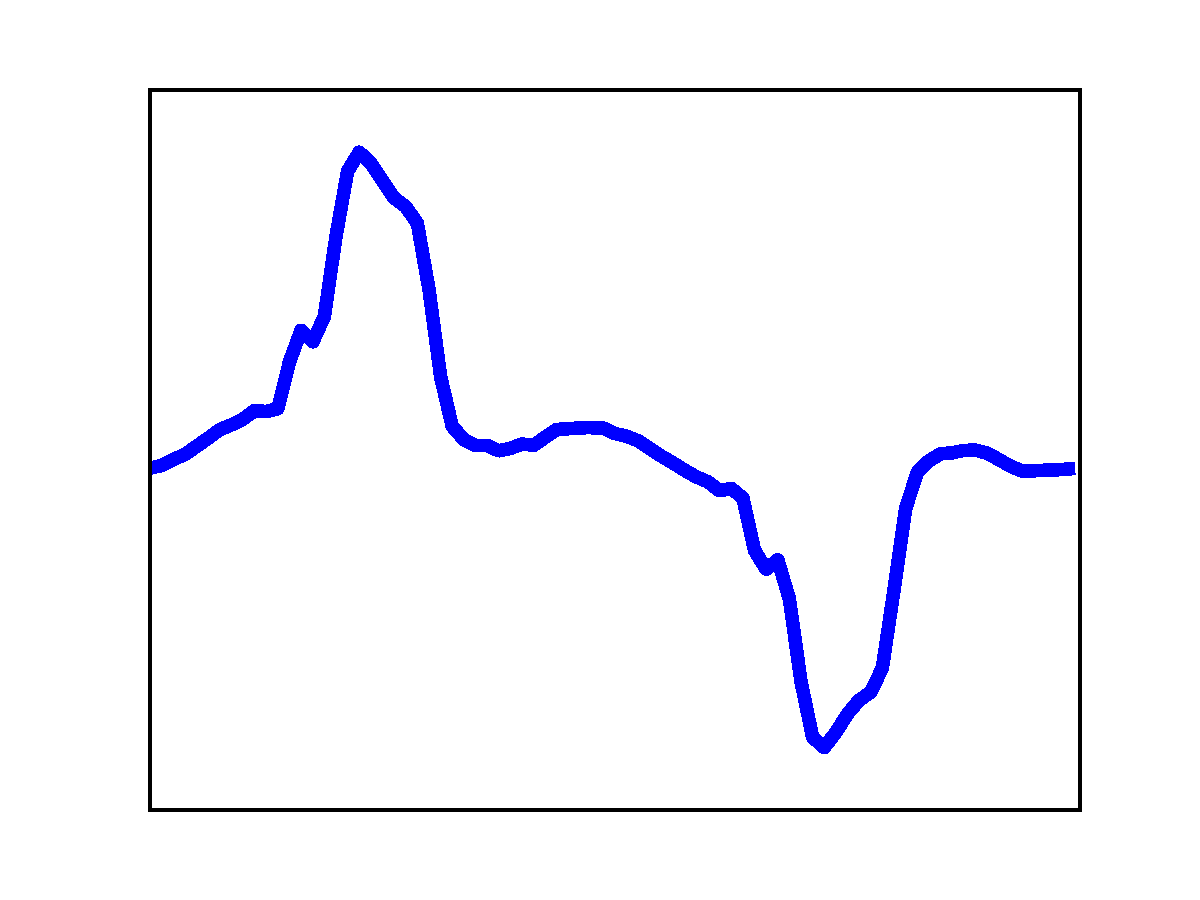
\includegraphics[width=20mm]{comps/comp_all50.pdf} 

\end{tabular}
\caption[BOLT: The components that contributed most to the disaggregation of the respective appliances.]{The components that contributed most to the disaggregation of the respective appliances.}
\label{waveforms}
\end{table}
The Boolean Re-Aggregation allows the recovery of the components which contributed most to the disaggregation of the appliances. Table \ref{waveforms} shows the three most influential components for some of the appliances excluding components that are connected by $\neg \land$, i.e. only appliances that have a positive influence on disaggregation. What is surprising is that, for example, the first waveform inferred for AV-LR seems to be more similar to the waveforms of the Computer than to its other waveforms. Since ground truth of the waveforms of the appliances is not available, it is unclear why this is the case. One possible explanation is that the algorithm exploited appliance co-variance information, i.e. if an appliance is only active when another appliance is active, the algorithm might learn the waveform of that other appliance.

\subsection{Unsupervised}
Table \ref{results_unsup} shows the results of the unsupervised approaches. The dataset is heavily biased towards some appliances, i.e. some appliances are active for just a fraction of the dataset. This bias seems to be reflected in the performance of the unsupervised disaggregation: only appliances that were active for at least 15\% achieved an F1 score of over 0.6. Even though the performance dropped substantially in comparison to the supervised case, it still seems to perform well in comparison to existing energy disaggregation algorithms. It is hard to compare different NILM systems since different algorithms are evaluated on different datasets. But to give an intuition on how well BOLT performs in comparison to other systems, we compared BOLT to the algorithm proposed in \cite{jiafully}. In \cite{jiafully} a disaggregation system based on non-parametric FHMMs is introduced and evaluated on the REDD \cite{kolter2011redd} dataset. REDD is of comparable complexity but the high-frequency portion of the dataset is compressed in a lossy way which might have a detrimental effect on the performance of BOLT. Their proposed method based on NFHMM achieves a score of 0.25 (GSPA, 0 worst, 1 best) on the REDD dataset in comparison to 0.61 unsupervised BOLT on the BLUED dataset.\\
For the na\"ive unsupervised re-aggregation, the optimal parameters $\lambda$ and $\epsilon$ were obtained for every appliance using cross-validation. The na\"ive unsupervised re-aggregation was only able to slightly improve the performance on a small subset of the appliances but it shows that it seems to be possible to further improve the unsupervised approach.

\begin{table}[]
\setlength{\tabcolsep}{3pt}
\centering
\begin{tabular}{lccccc}
\hline
Appliance      & Active            & Lower Bound F1 & Na\"ive F1 \\ \hline
A/V LR         & 60\%              & 0.85        & 0.85         \\
Computer 1     & 27.3\%            & 0.67        & 0.74      \\
Desk Lamp      & 21.4\%            & 0.70        & 0.70     \\
DVR            & 20.7\%            & 0.85         & 0.85      \\
Socket LR      & $>0.1\%$ & 0.0       & 0.0      \\
Garage Door    & 0.4 \%            & 0.24          & 0.3  \\
Iron           & 0.1 \%            & 0.09        & 0.30   \\
Laptop 1       & 33.3\%            & 0.71        & 0.71   \\
LCD Monitor    & 16.2\%            & 0.63        & 0.63  \\
Monitor 2      & 17.3\%            & 0.67        & 0.70  \\
Printer        & 0.1\%             & 0.07           & 0.07 \\
Tall Desk Lamp & 21.4\%            & 0.70        & 0.70   \\
TV Basement    & 20.7\%            & 0.85        & 0.85   \\ \hline
\end{tabular}
\caption[BOLT: Unsupervised performance comparison]{ ``Lower Bound F1'' and ``Na\"ive F1'' show the performance using different unsupervised reaggregation techniques.}
\label{results_unsup}
\end{table}

\newpage
\section{Hardware Implementation}

\begin{figure}[!ht]
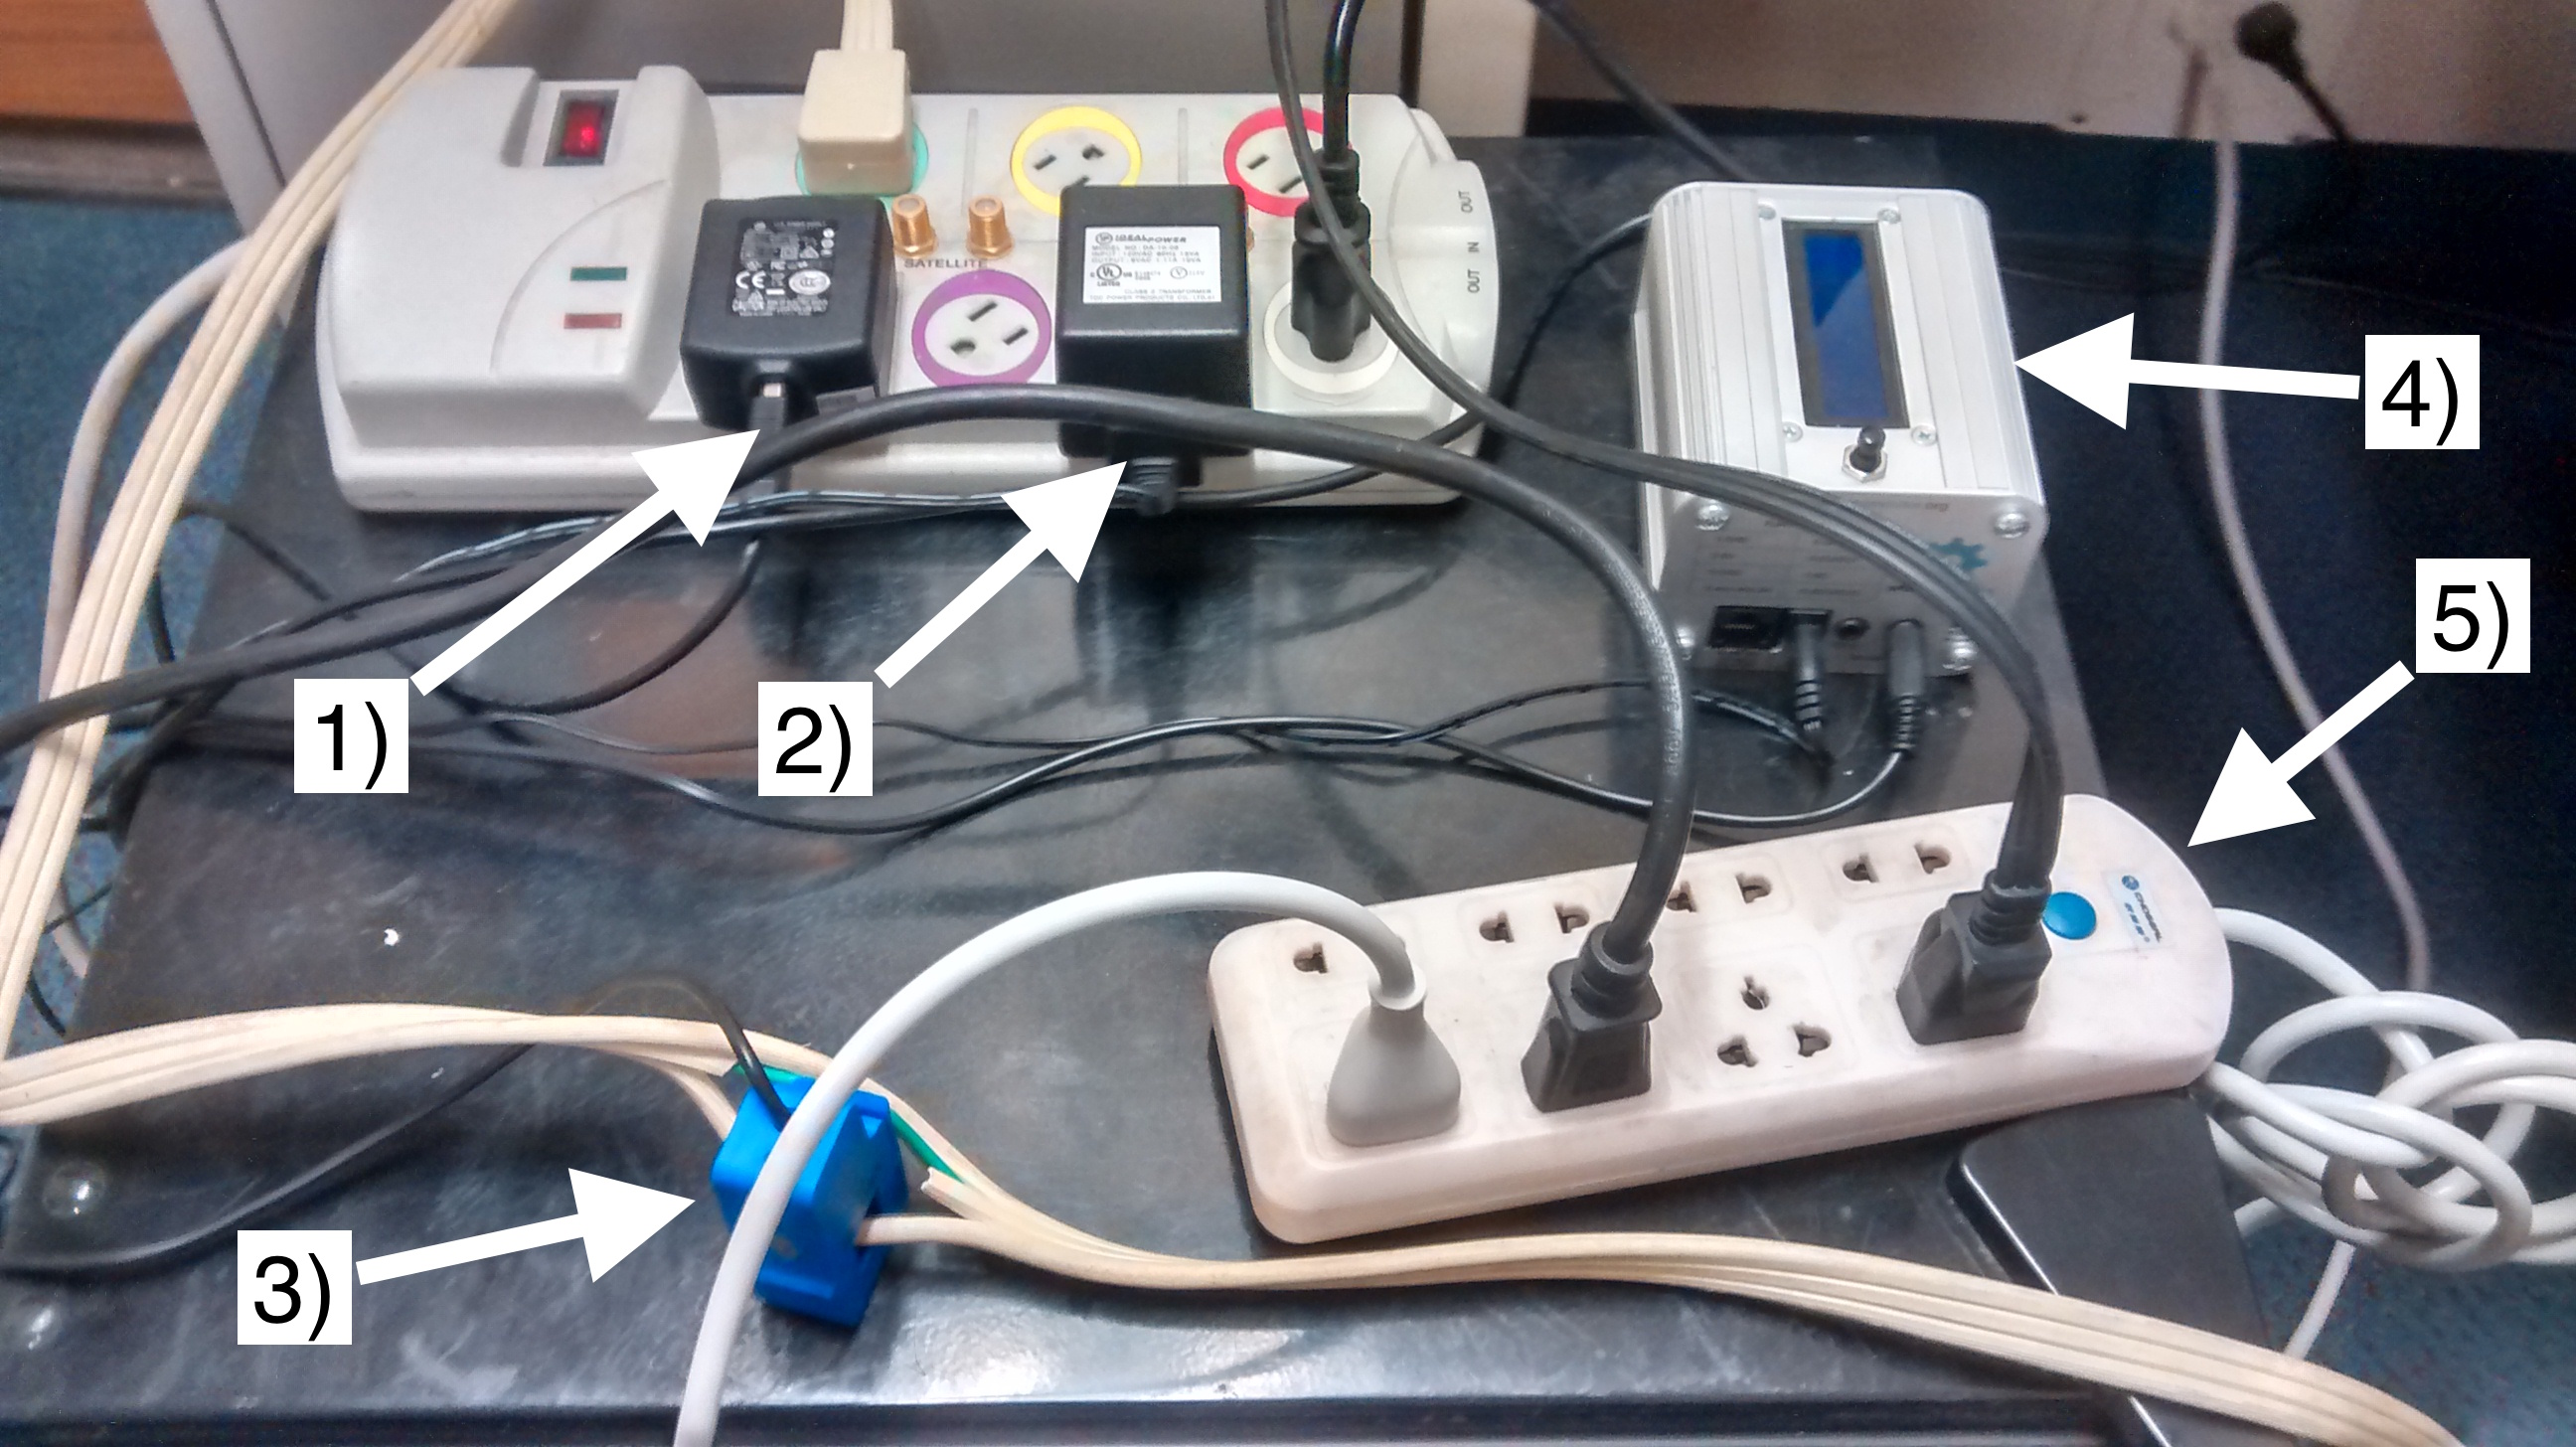
\includegraphics[width=0.85\linewidth]{bolt/OEM.jpg}
\caption[BOLT: The OpenEnergyMonitor setup.]{1.) Voltage Input, 2.) Power Supply, 3.) Current Transformer 4.) OpenEnergyMonitor 5.) Metered Power Strip }
\label{fg:oem}
\end{figure}

NILM systems that rely on high sampling rates of the current or voltage signal quickly run into data transmission and storage problems. For example, a system which carries out inference on a centralized server and that requires a sampling rate of 12kHz would need to transmit and store approximately 4GB per sensor day assuming a sensor resolution of 16bits per sample. Such a system would not scale well to many sensors (or buildings). \ourname, however, can infer the states of the subcomponents directly and then only transmit these states. Since the states of the subcomponents can be encoded by a single bit per subcomponent, inferring the subcomponents can be viewed as very strong compression and, as we have shown earlier, this compression preserves the information of appliance activities. By doing so, the data that needs to be transmitted can be reduced to 8.5MB per sensor/day, resulting in a 500 fold reduction.\\
Ultimately, the data that needs to be transmitted is independent of the internal sampling frequency and only depends on the number of subcomponents. This means that theoretically, megahertz sampling frequencies could be leveraged while still keeping the data transmission and storage costs low. However practically, with increasing internal sampling frequency, the computational burden increases which in turn requires computationally more powerful smart-metering hardware.\\
We conducted an experiment to show the maximum sampling rates achievable with a Raspberry Pi 2\footnote{http://raspberrypi.org}. Figure \ref{fg:oem} shows a picture of the experimental setup. The Raspberry Pi is a ubiquitous, low-cost (US \$35) embedded computing platform powered by a 900MHz quad-core ARM Cortex-A7. The open source Open Energy Monitor\footnote{http://openenergymonitor.org} was used for our experiments. The Raspberry Pi built into the Open Energy Monitor is internally connected to a micro-controller powered by an ATMega328p with an internal clock rate of 16MHz which serves as a sensing relay.

\begin{figure}[!ht]
\centering
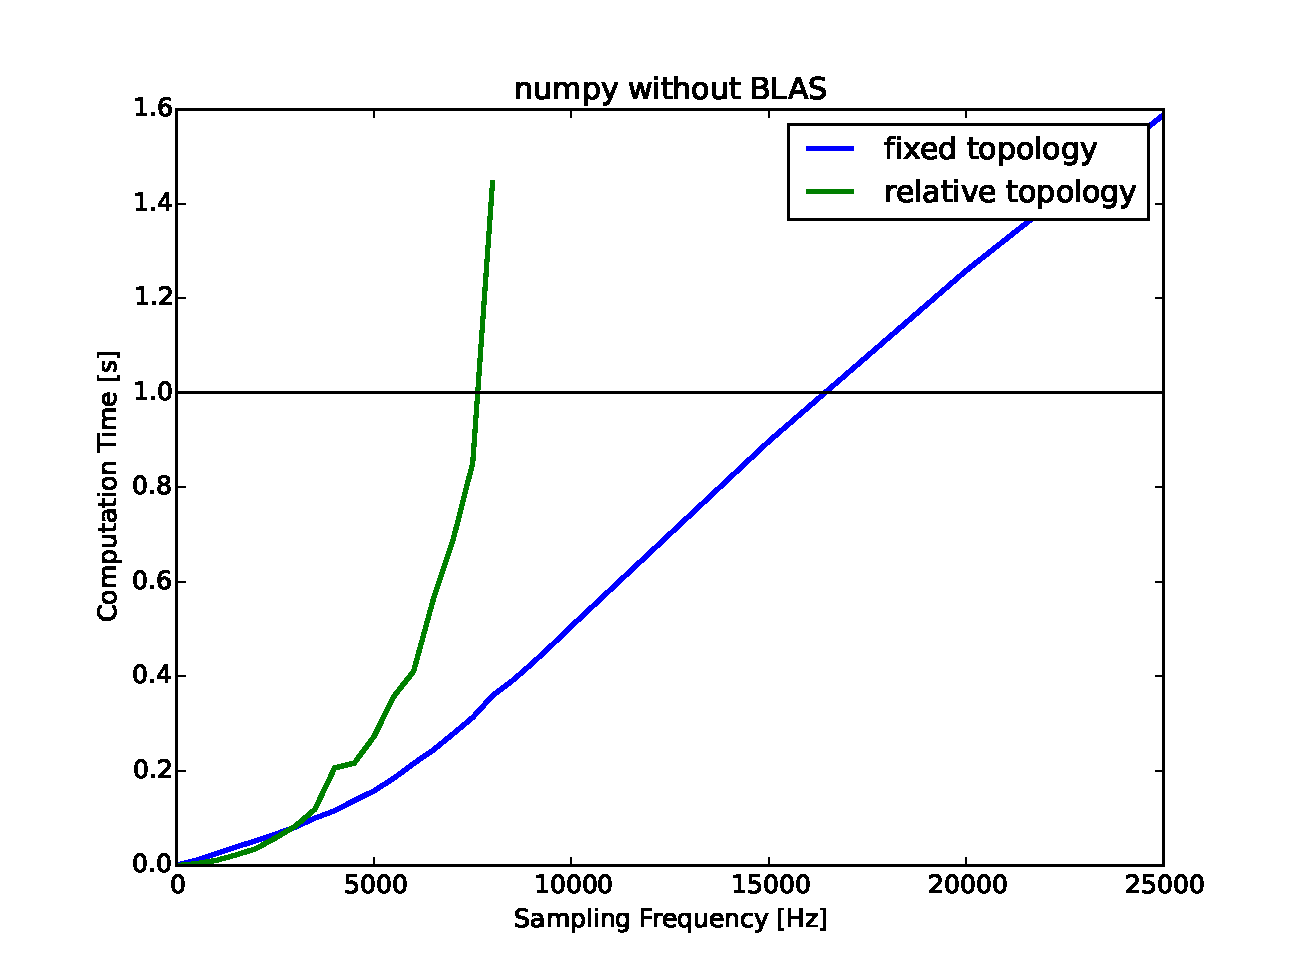
\includegraphics[width=0.75\linewidth]{bolt/sampling_freq.eps}
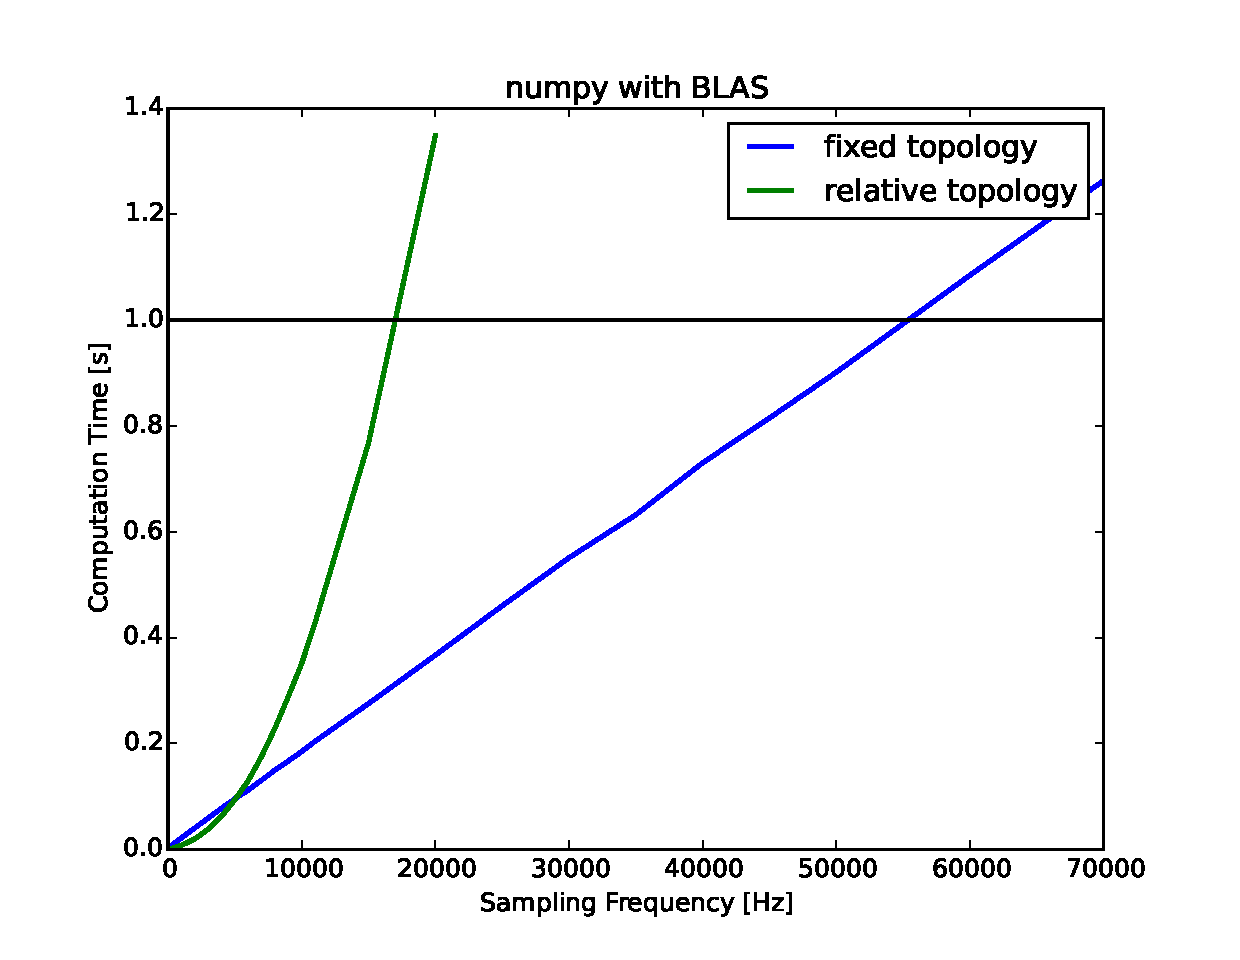
\includegraphics[width=0.75\linewidth]{bolt/sampling_freq_blas.eps}
\caption[BOLT: Computational time as a function of the sampling rate.]{The computational time as a function of the sampling rate. The top figure assumes a simple numpy implementation whereas the bottom figure uses numpy and BLAS. The black horizontal line marks up until when real time inference is possible.}
\label{fig_imp}
\end{figure}

The computational cost of inferring the states of the subcomponents is a function of the number of computational nodes in the network and by increasing the sampling frequency, at the very least, the number of the computational nodes in the input layer increases. In order to investigate the limits of real-time inference as a function of the sampling rate two sets of experiments were conducted. In the first experiment a fixed topology of the network is assumed: Let $f$ be the sampling rate. The topology of the network is in the first experiment: $f \rightarrow 500 \rightarrow 100 \rightarrow f$, i.e. there are $f$ input neurons that project the input onto a hidden layer consisting of 500 neurons which in turn projects the input down onto 100 binary units. The states of the binary units in turn are used to recreate the input, i.e. the output dimensionality is also $f$. In the second experiment, we considered a network whose topology grows linearly with the sampling rate. Data with a higher sampling rate might contain more structure and in turn require more flexibility of the network to disaggregate the waveforms. The topology of the `relative network' is set to: $f \rightarrow f/10 \rightarrow 100 \rightarrow f$. Inference is carried out with an implementation using the Python package numpy. Since inference in neural networks can be implemented by a succession of matrix-multiplications followed by the application of a non-linearity, the potential speed-up by using BLAS (Basic Linear Algebra Subprograms\footnote{http://www.netlib.org/blas/}) is also investigated.\\
Note that with a simple trick, the costs of having to transform the inputs into frequency domain during inference, i.e. the costs of the FFT can be avoided by exploiting the linearity of the matrix-multiplications and FFT. Let $y(t)$ be the input at time $t$ and $w$ be the first column of the weights coming into the first layer. Let $\mathcal{F}$ denote the Fourier transform, i.e. $\mathcal{F}(y(t))_k = \sum_{j=0}^N exp(-2\pi jk/N)y(t)_j$. For the activation of the first neuron in the first layer before applying the non-linearity the following holds: 
\begin{align*}
\mathcal{F}(y(t))^Tw &=\sum_{k=0}^N w_k \sum_{j=0}^N exp(-2\pi jk/N)y(t)_j\\
 &=\sum_{k=0}^N y(t)_k \sum_{j=0}^N exp(-2\pi jk/N) w_j = \mathcal{F}(w)^Ty(t)
\end{align*}
 This ultimately means that instead of computing the Fourier Transform of every input, instead the Fourier transform of the weight-matrix can be computed once leading to a substantial decrease in computational cost. Training the network in frequency-domain and doing inference in time-domain allows for enforcing frequency-constraints while at the same time keeping the computational time needed for inference low.\\
Figure \ref{fig_imp} shows the increase in computational time as a function of the sampling rate for the topologies described above. The top figure shows the inference time using a simple numpy implementation whereas the bottom figure shows a numpy implementation using BLAS. The sampling frequency describes the data collected within 1 second and as long as the data collected can be processed in less than 1s, real time inference is possible on the smart meter. It can be seen that when using a fixed topology, real-time inference using BLAS is possible up until sampling rates of 55kHz. But as we have shown earlier, even a sampling rate of only 4.8kHz suffices to infer appliance states with high precision.

\section{Conclusion}

The approach introduced in this paper seems to be the first approach that acknowledges the fact that loads are not necessarily linear, i.e. not all loads are phase-shifted sinusoids. Most approaches simply use active and reactive power as features and neglect the fact that some appliances have very distinct waveforms which cannot be characterized in the traditional resistive, inductive and capacitive load trichotomy. Applying Binary Matrix Factorization in order to infer reoccurring additive subcomponents in the current signal allows to decompose the current signal and extract a very rich set of features: component waveforms. Combining the inferred components to ultimately infer whether or not an appliance is active has shown great potential. The supervised case approaches what is theoretically possible under the assumption of 2-state appliances but requires the availability of training data whereas the results of unsupervised approaches indicate the possibility of re-aggregating appliances in an unsupervised way.\\ The approach introduced in this paper also shows advantages from a computation point of view: the hidden state given some input can be viewed as a drastically compressed representation of the input that preserves information about which appliances are active and, since inference of the hidden states using the neural network is computationally cheap, only the hidden states (component states) need to be transmitted, which in turn reduces the data storage and transmission burden while still leveraging high-frequency information. For instance, an approach that requires remote inference and a sampling frequency of 12kHz would need to send out 96kb/s as opposed to 16byte/s (100bits per component + 32bits for the aggregate signal) using this approach. Additionally, inferring which appliances are active at any given time requires only a 1 second slice of current, which in turn implies that inference can be carried out without the need of a warm-up phase such as those required by approaches based on FHMM.

\section{Future work}

Some machine learning systems such as, for example, a system that predicts the future value of a random variable in can continuously learn from its mistakes. In order to obtain the information of whether or not a past prediction was right or wrong, simply time needs to pass and the correct value can be observed. In this respect, NILM systems face an additional difficulty: a purely non-intrusive system can never learn from its mistakes because it cannot observe the true state of appliances. This characteristic is detrimental for supervised approaches that assume snapshot knowledge of appliances because, implicitly, these approaches also assume that loads do not change over time. For unsupervised approaches, this means that the entire NILM system can only be evaluated on a minuscule subset of homes which are submetered and buildings for which the systems performs suboptimally can at most only tried to be identified by indirect metrics. Because of the unsupervised nature of the subcomponent identification step of the system introduced in this paper, continuous retraining of the system is possible. However, combining the subcomponents into appliances still requires training to allow for high precision disaggregation. The requirement for training can, nonetheless, be alleviated. Two strategies that might alleviate the need for ground truth will be discussed here in more detail.
\begin{description}
\item[Sparse Coding and Waveform Library] As we have discussed earlier, especially in the unsupervised case, the proposed system struggles with purely resistive loads as they lack discriminative features. The algorithm can always stitch together and re-use sinusoids. This problem could however be alleviated by enforcing sparsity of the binary hidden layer of the neural network. If the algorithm stitches sinusoids together, more subcomponents are active in comparison to a scenario in which each subcomponent represents an appliance. This is why the effect of enforcing sparsity in the hidden layer of the neural network might be worth investigating.\\
Enforcing sparsity in the hidden layer is closely linked with infusing prior knowledge into the system. If knowledge about the appliances present in a building is assumed, this knowledge could be used to alleviate the need for ground truth. In case the waveforms of the appliance are known, i.e. the algorithm can access a waveform library that contains the waveforms of individual appliances, a prior distribution over the weights coming into the output layer (the component waveforms) could be imposed in order to enforce that the component waveforms are similar to the elements in the waveform library.
\item[Distributed Sensing] Another way to alleviate the need for ground truth is to build a hybrid approach. For some chain franchises like e.g. fast food restaurants, gas stations, supermarkets, etc. the assumption that loads are similar across different buildings might be valid. This could be leveraged by submetering a subset of the franchise locations and broadcasting the appliance specifics knowledge from the submetered to the non-submetered locations. BOLT seems to be a prime candidate for such a strategy since the subcomponent identification portion of the algorithm is unsupervised. This allows to fuse the data collected at all franchise locations into a single stream of data. This stream of data can then in turn be used to train the unsupervised neural network model. In order to infer appliance states of non-submetered locations, the data at the submetered locations can be leveraged to create a supervised model which is then shared with the non-submetered locations. Such a strategy has many advantages over traditional NILM systems: 
\begin{itemize}
\item Continuous re-training allows handling of load patterns that might change over time
\item Potentially high precision NILM while still bringing down the costs substantially - only a small subset locations would need to be submetered
\item Training a joint unsupervised model of all franchise locations allows to incorporate information of non-submetered locations into the modeling process which might make the overall system very robust
\item Deep Learning seems to thrive on big datasets and in such a scenario BOLT could in principle leverage the information of an infinite data stream
\end{itemize}
Such a distributed NILM system however creates new challenges. For example, the system needs to communicate information between different smart meters extensively. Whether BOLT can be used to reduce the data transmission requirements is an interesting future research direction, especially as technologies like Low Power Wide Area Networks (LP-WAN) become more widespread.
\end{description}